% Options for packages loaded elsewhere
\PassOptionsToPackage{unicode}{hyperref}
\PassOptionsToPackage{hyphens}{url}
%
\documentclass[
  oneside]{book}
\usepackage{amsmath,amssymb}
\usepackage{iftex}
\ifPDFTeX
  \usepackage[T1]{fontenc}
  \usepackage[utf8]{inputenc}
  \usepackage{textcomp} % provide euro and other symbols
\else % if luatex or xetex
  \usepackage{unicode-math} % this also loads fontspec
  \defaultfontfeatures{Scale=MatchLowercase}
  \defaultfontfeatures[\rmfamily]{Ligatures=TeX,Scale=1}
\fi
\usepackage{lmodern}
\ifPDFTeX\else
  % xetex/luatex font selection
\fi
% Use upquote if available, for straight quotes in verbatim environments
\IfFileExists{upquote.sty}{\usepackage{upquote}}{}
\IfFileExists{microtype.sty}{% use microtype if available
  \usepackage[]{microtype}
  \UseMicrotypeSet[protrusion]{basicmath} % disable protrusion for tt fonts
}{}
\makeatletter
\@ifundefined{KOMAClassName}{% if non-KOMA class
  \IfFileExists{parskip.sty}{%
    \usepackage{parskip}
  }{% else
    \setlength{\parindent}{0pt}
    \setlength{\parskip}{6pt plus 2pt minus 1pt}}
}{% if KOMA class
  \KOMAoptions{parskip=half}}
\makeatother
\usepackage{xcolor}
\usepackage[margin=1in]{geometry}
\usepackage{color}
\usepackage{fancyvrb}
\newcommand{\VerbBar}{|}
\newcommand{\VERB}{\Verb[commandchars=\\\{\}]}
\DefineVerbatimEnvironment{Highlighting}{Verbatim}{commandchars=\\\{\}}
% Add ',fontsize=\small' for more characters per line
\usepackage{framed}
\definecolor{shadecolor}{RGB}{248,248,248}
\newenvironment{Shaded}{\begin{snugshade}}{\end{snugshade}}
\newcommand{\AlertTok}[1]{\textcolor[rgb]{0.94,0.16,0.16}{#1}}
\newcommand{\AnnotationTok}[1]{\textcolor[rgb]{0.56,0.35,0.01}{\textbf{\textit{#1}}}}
\newcommand{\AttributeTok}[1]{\textcolor[rgb]{0.13,0.29,0.53}{#1}}
\newcommand{\BaseNTok}[1]{\textcolor[rgb]{0.00,0.00,0.81}{#1}}
\newcommand{\BuiltInTok}[1]{#1}
\newcommand{\CharTok}[1]{\textcolor[rgb]{0.31,0.60,0.02}{#1}}
\newcommand{\CommentTok}[1]{\textcolor[rgb]{0.56,0.35,0.01}{\textit{#1}}}
\newcommand{\CommentVarTok}[1]{\textcolor[rgb]{0.56,0.35,0.01}{\textbf{\textit{#1}}}}
\newcommand{\ConstantTok}[1]{\textcolor[rgb]{0.56,0.35,0.01}{#1}}
\newcommand{\ControlFlowTok}[1]{\textcolor[rgb]{0.13,0.29,0.53}{\textbf{#1}}}
\newcommand{\DataTypeTok}[1]{\textcolor[rgb]{0.13,0.29,0.53}{#1}}
\newcommand{\DecValTok}[1]{\textcolor[rgb]{0.00,0.00,0.81}{#1}}
\newcommand{\DocumentationTok}[1]{\textcolor[rgb]{0.56,0.35,0.01}{\textbf{\textit{#1}}}}
\newcommand{\ErrorTok}[1]{\textcolor[rgb]{0.64,0.00,0.00}{\textbf{#1}}}
\newcommand{\ExtensionTok}[1]{#1}
\newcommand{\FloatTok}[1]{\textcolor[rgb]{0.00,0.00,0.81}{#1}}
\newcommand{\FunctionTok}[1]{\textcolor[rgb]{0.13,0.29,0.53}{\textbf{#1}}}
\newcommand{\ImportTok}[1]{#1}
\newcommand{\InformationTok}[1]{\textcolor[rgb]{0.56,0.35,0.01}{\textbf{\textit{#1}}}}
\newcommand{\KeywordTok}[1]{\textcolor[rgb]{0.13,0.29,0.53}{\textbf{#1}}}
\newcommand{\NormalTok}[1]{#1}
\newcommand{\OperatorTok}[1]{\textcolor[rgb]{0.81,0.36,0.00}{\textbf{#1}}}
\newcommand{\OtherTok}[1]{\textcolor[rgb]{0.56,0.35,0.01}{#1}}
\newcommand{\PreprocessorTok}[1]{\textcolor[rgb]{0.56,0.35,0.01}{\textit{#1}}}
\newcommand{\RegionMarkerTok}[1]{#1}
\newcommand{\SpecialCharTok}[1]{\textcolor[rgb]{0.81,0.36,0.00}{\textbf{#1}}}
\newcommand{\SpecialStringTok}[1]{\textcolor[rgb]{0.31,0.60,0.02}{#1}}
\newcommand{\StringTok}[1]{\textcolor[rgb]{0.31,0.60,0.02}{#1}}
\newcommand{\VariableTok}[1]{\textcolor[rgb]{0.00,0.00,0.00}{#1}}
\newcommand{\VerbatimStringTok}[1]{\textcolor[rgb]{0.31,0.60,0.02}{#1}}
\newcommand{\WarningTok}[1]{\textcolor[rgb]{0.56,0.35,0.01}{\textbf{\textit{#1}}}}
\usepackage{longtable,booktabs,array}
\usepackage{calc} % for calculating minipage widths
% Correct order of tables after \paragraph or \subparagraph
\usepackage{etoolbox}
\makeatletter
\patchcmd\longtable{\par}{\if@noskipsec\mbox{}\fi\par}{}{}
\makeatother
% Allow footnotes in longtable head/foot
\IfFileExists{footnotehyper.sty}{\usepackage{footnotehyper}}{\usepackage{footnote}}
\makesavenoteenv{longtable}
\usepackage{graphicx}
\makeatletter
\def\maxwidth{\ifdim\Gin@nat@width>\linewidth\linewidth\else\Gin@nat@width\fi}
\def\maxheight{\ifdim\Gin@nat@height>\textheight\textheight\else\Gin@nat@height\fi}
\makeatother
% Scale images if necessary, so that they will not overflow the page
% margins by default, and it is still possible to overwrite the defaults
% using explicit options in \includegraphics[width, height, ...]{}
\setkeys{Gin}{width=\maxwidth,height=\maxheight,keepaspectratio}
% Set default figure placement to htbp
\makeatletter
\def\fps@figure{htbp}
\makeatother
\setlength{\emergencystretch}{3em} % prevent overfull lines
\providecommand{\tightlist}{%
  \setlength{\itemsep}{0pt}\setlength{\parskip}{0pt}}
\setcounter{secnumdepth}{5}
\usepackage{booktabs}

\usepackage{tcolorbox}
\usepackage[T1]{fontenc}

\definecolor{dangcol}{RGB}{152,62,130}
\definecolor{warncol}{RGB}{245,220,112}
\definecolor{infocol}{RGB}{70,122,172}
\definecolor{trycol}{RGB}{97,88,156}

\newtcolorbox{dangerous}{
  colback=dangcol!10,
  colframe=dangcol,
  coltext=black,
  boxsep=5pt,
  arc=4pt
}

\newtcolorbox{warning}{
  colback=warncol!10,
  colframe=warncol,
  coltext=black,
  boxsep=5pt,
  arc=4pt
}

\newtcolorbox{info}{
  colback=infocol!10,
  colframe=infocol,
  coltext=black,
  boxsep=5pt,
  arc=4pt
}

\newtcolorbox{try}{
  colback=trycol!10,
  colframe=trycol,
  coltext=black,
  boxsep=5pt,
  arc=4pt
}
\usepackage{booktabs}
\usepackage{longtable}
\usepackage{array}
\usepackage{multirow}
\usepackage{wrapfig}
\usepackage{float}
\usepackage{colortbl}
\usepackage{pdflscape}
\usepackage{tabu}
\usepackage{threeparttable}
\usepackage{threeparttablex}
\usepackage[normalem]{ulem}
\usepackage{makecell}
\usepackage{xcolor}
\ifLuaTeX
  \usepackage{selnolig}  % disable illegal ligatures
\fi
\usepackage[]{natbib}
\bibliographystyle{plainnat}
\usepackage{bookmark}
\IfFileExists{xurl.sty}{\usepackage{xurl}}{} % add URL line breaks if available
\urlstyle{same}
\hypersetup{
  pdftitle={Intro to Data Viz Using R},
  pdfauthor={Emily Nordmann},
  hidelinks,
  pdfcreator={LaTeX via pandoc}}

\title{Intro to Data Viz Using R}
\author{Emily Nordmann}
\date{2025-03-28}

\begin{document}
\maketitle

{
\setcounter{tocdepth}{1}
\tableofcontents
}
\chapter*{Overview}\label{overview}
\addcontentsline{toc}{chapter}{Overview}

To get the most out of the webinar, you should have R and RStudio installed so that you can follow along and execute the code on your own device. You don't have to do this and you are welcome to just listen in but you will get more out of the session if you play an active role.

\begin{itemize}
\tightlist
\item
  If you don't currently have R or RStudio installed, we have produced a guide on how to install R and Rstudio \href{https://psyteachr.github.io/RSetGo/installing-r-windows.html}{for Windows} and for \href{https://psyteachr.github.io/RSetGo/installing-r-mac.html}{Mac}.
\item
  If you have R and/or RStudio installed, you can follow \href{https://psyteachr.github.io/RSetGo/updating-r.html}{this guide to update} to the latest version before the workshop.
\item
  If you have technical issues and cannot install R and RStudio on your machine (e.g., if you don't have admin rights), you can sign-up for an \href{https://rstudio.cloud/}{RStudio Cloud} account although the interface will be a little different from the desktop version that will be used in the webinar.
\item
  Please note that I will not be able to provide technical assistance during the webinar for installation issues.
\end{itemize}

Once you've done one of the above:

\begin{itemize}
\tightlist
\item
  Work through Chapter~\ref{intro} which will introduce you to some basic programming terminology and install everything you need to follow along in the workshop. Depending upon your familiarity with R, this should take 1-2 hours.
\item
  Familiarize yourself with the data set we'll be using for this webinar by reading the associated paper \href{https://openpsychologydata.metajnl.com/articles/10.5334/jopd.80}{Data from an International Multi-Centre Study of Statistics and Mathematics Anxieties and Related Variables in University Students (the SMARVUS Dataset)}
\item
  Download the data files - here is a zip folder of everything you need. Unzip the folder and have a look through the Rmd files - these are the ones we'll use in the webinar.
\item
  Browse through the FAQs for responses to questions submitted in advance of the webinar that includes links to additional training and materials for learning R.
\end{itemize}

\section{Statement on AI use}\label{statement-on-ai-use}

This webinar and online resource was designed by a human (Emily Nordmann) but augmented with the use of ChatGPT4o.

\chapter{Intro to R and RStudio}\label{intro}

\section{Intended Learning Outcomes}\label{ilo-intro}

By the end of this chapter, learners should be able to:
* Install R and RStudio
* Install add-on packages
* Get help for packages and functions
* Create objects by writing and running code in the console

Please note that if you're completely new to R, we don't expect you to fully understand everything in this chapter and getting comfortable with coding does take continued practice. However, you will get more out of the webinar if you have some familiarity with the basics.

Download the \href{https://raw.githubusercontent.com/rstudio/cheatsheets/main/rstudio-ide.pdf}{RStudio IDE Cheatsheet}.

\section{R and RStudio}\label{intro-r-rstudio}

R is a programming language that you will write code in and RStudio is an Integrated Development Environment (IDE{}) which makes working in R easier. Think of it as knowing English and using a plain text editor like NotePad to write a book versus using a word processor like Microsoft Word. You could do it, but it would be much harder without things like spell-checking and formatting and you wouldn't be able to use some of the advanced features that Word has developed. In a similar way, you can use R without R Studio but we wouldn't recommend it. RStudio serves as a text editor, file manager, spreadsheet viewer, and more. The key thing to remember is that although you will do all of your work using RStudio for this workshop, you are actually using two pieces of software which means that from time-to-time, both of them may have separate updates.

\subsection{RStudio}\label{rstudio_ide}

When you installed R, that gave your computer the ability to process the R programming language, and also installed an app called ``R''. We will never use that app. Instead, we will use \href{http://www.rstudio.com}{RStudio}. RStudio is arranged with four window panes{}.

\begin{figure}

{\centering 
\includegraphics[width=1\linewidth]{images/intro/rstudio} 

}

\caption{The RStudio IDE}\label{fig:img-rstudio}
\end{figure}

By default, the upper left pane is the \textbf{source pane}, where you view, write, and edit code from files and view data tables in a spreadsheet format. When you first open RStudio, this pane won't display until we open a document or load in some data - don't worry, we'll get to that soon.

The lower left pane is the \textbf{console pane}, where you can type in commands and view output messages. You can write code in the console to test it out. The code will run and can create objects in the environment, but the code itself won't be saved. You need to write your code into a script in the source pane to save it.

The right panes have several different tabs that show you information about your code. The most used tabs in the upper right pane are the \textbf{Environment} tab and the \textbf{Help} tab. The environment tab lists some information about the objects{} that you have defined in your code. We'll learn more about the Help tab in Section~\ref{function-help}.

In the lower right pane, the most used tabs are the \textbf{Files} tab for directory structure, the \textbf{Plots} tab for plots made in a script, the \textbf{Packages} tab for managing add-on packages (see Section~\ref{packages}), and the \textbf{Viewer} tab to display reports created by your scripts. You can change the location of panes and what tabs are shown under \textbf{\texttt{Preferences\ \textgreater{}\ Pane\ Layout}}.

\subsection{Reproducibility}\label{intro-reproducibility}

One of the main reasons to learn R is that you can create reproducible{} reports. This involves writing scripts that transform data, create summaries and visualisations, and embed them in a report in a way that always gives you the same results.

When you do things reproducibly, others (and future you) can understand and check your work. You can also reuse your work more easily. For example, if you need to create the same exam board report every semester for student grades, a reproducible report allows you to download the new data and create the report within seconds. It might take a little longer to set up the report in the first instance with reproducible methods, but the time it saves you in the long run is invaluable.

\begin{try}

Section~\ref{rstudio-settings} shows you how to change two important settings in the global Options to increase reproducibility. Your settings should have:

\begin{itemize}
\item
  Restore .RData into workspace at startup:
\item
  \begin{enumerate}
  \def\labelenumi{(\Alph{enumi})}
  \tightlist
  \item
    Checked\\
  \end{enumerate}
\item
  \begin{enumerate}
  \def\labelenumi{(\Alph{enumi})}
  \setcounter{enumi}{1}
  \tightlist
  \item
    Not Checked
  \end{enumerate}
\item
  Save workspace to .RData on exit:
\item
  \begin{enumerate}
  \def\labelenumi{(\Alph{enumi})}
  \tightlist
  \item
    Always\\
  \end{enumerate}
\item
  \begin{enumerate}
  \def\labelenumi{(\Alph{enumi})}
  \setcounter{enumi}{1}
  \tightlist
  \item
    Never\\
  \end{enumerate}
\item
  \begin{enumerate}
  \def\labelenumi{(\Alph{enumi})}
  \setcounter{enumi}{2}
  \tightlist
  \item
    Ask
  \end{enumerate}
\end{itemize}

\end{try}

\subsection{Themes and accessiblilty}\label{themes-and-accessiblilty}

You can customise how R Studio looks to make it work for you. Click \texttt{Tools} - \texttt{Global\ Options} - \texttt{Appearance}. You can change the default font, font size, and general appearance of R Studio, including using dark mode. Play around with the settings and see what you prefer - you're going to spend a lot of time with R, it might as well look nice!

\section{Sessions}\label{intro-sessions}

If you have the above settings configured correctly, when you open up RStudio and start writing code, loading packages, and creating objects, you will be doing so in a new session and your Environment tab should be completely empty. If you find that your code isn't working and you can't figure out why, it might be worth restarting your R session. This will clear the environment and detach all loaded packages - think of it like restarting your phone. There are several ways that you can restart R:

\begin{itemize}
\tightlist
\item
  Menu: Session \textgreater{} Restart R
\item
  {Cmd-Shift-F10} or {Ctl-Shift-F10}
\item
  type \texttt{.rs.restartR()} in the console
\end{itemize}

Try doing each of these now. Additionally, now would be a good time to create a notebook where you can keep a record of useful hints and tips and things to try when your code isn't working. Add ``restart R session'' to this notebook as your first item.

\section{Functions}\label{functions}

When you install R you will have access to a range of functions{} including options for data wrangling{} and statistical analysis. The functions that are included in the default installation are typically referred to as base R{} and you can think of them like the default apps that come pre-loaded on your phone.

A function{} is a name that refers to some code you can reuse. We'll be using functions that are provided in packages, but you can also write your own functions.

If you type a function into the console pane, it will run as soon as you hit enter. If you put the function in a script{} or R Markdown{} document in the source pane{}, it won't run until you run the script, knit{} the R Markdown file, or run a code chunk{}. You'll learn more about this in the workshop.

For example, the function \texttt{sum()} is included in base R, and does what you would expect. In the console, run the below code:

\begin{Shaded}
\begin{Highlighting}[]
\FunctionTok{sum}\NormalTok{(}\DecValTok{1}\NormalTok{,}\DecValTok{2}\NormalTok{,}\DecValTok{3}\NormalTok{)}
\end{Highlighting}
\end{Shaded}

\begin{verbatim}
## [1] 6
\end{verbatim}

\section{Packages}\label{packages}

One of the great things about R, however, is that it is \textbf{user extensible}: anyone can create a new add-on that extends its functionality. There are currently thousands of packages{} that R users have created to solve many different kinds of problems, or just simply to have fun. For example, there are packages for data visualisation, machine learning, interactive dashboards, web scraping, and playing games such as Sudoku.

Add-on packages are not distributed with base R, but have to be downloaded and installed from an archive, in the same way that you would, for instance, download and install PokemonGo on your smartphone. The main repository where packages reside is called CRAN{}, the Comprehensive R Archive Network.

There is an important distinction between \textbf{installing} a package and \textbf{loading} a package.

\subsection{Installing a package}\label{install-package}

This is done using {{install.packages}{(}{)}}. This is like installing an app on your phone: you only have to do it once and the app will remain installed until you remove it. For instance, if you want to use PokemonGo on your phone, you install it once from the App Store or Play Store; you don't have to re-install it each time you want to use it. Once you launch the app, it will run in the background until you close it or restart your phone. Likewise, when you install a package, the package will be available (but not \emph{loaded}) every time you open up R.

Install the tidyverse package on your system. This package is the main package we will use throughout this book for data wrangling, summaries, and visualisation.

\begin{Shaded}
\begin{Highlighting}[]
\CommentTok{\# type this in the console pane}
\FunctionTok{install.packages}\NormalTok{(}\StringTok{"tidyverse"}\NormalTok{)}
\end{Highlighting}
\end{Shaded}

If you get a message that says something like \texttt{package\ ‘tidyverse’\ successfully\ unpacked\ and\ MD5\ sums\ checked}, the installation was successful. If you get an error and the package wasn't installed, check the troubleshooting section of Appendix~\ref{package-install-troubleshooting}.

\begin{dangerous}
Never install a package from inside a script. Only do this from the console pane.

\end{dangerous}

You can also install multiple packages at once. Here is the command to install all of the packages we'll be using in this webinar

\begin{Shaded}
\begin{Highlighting}[]
\NormalTok{packages }\OtherTok{\textless{}{-}} \FunctionTok{c}\NormalTok{(}
  \StringTok{"tidyverse"}\NormalTok{,  }\CommentTok{\# for everything}
  \StringTok{"patchwork"}\NormalTok{,  }\CommentTok{\# for multi{-}part plots}
  \StringTok{"ggthemes"}\NormalTok{,   }\CommentTok{\# for themed plots}
  \StringTok{"devtools"}    \CommentTok{\# for installing github packages}
\NormalTok{)}

\CommentTok{\# determine which need to be installed}
\NormalTok{new\_packages }\OtherTok{\textless{}{-}}\NormalTok{ packages[}\SpecialCharTok{!}\NormalTok{packages }\SpecialCharTok{\%in\%} \FunctionTok{installed.packages}\NormalTok{()]}

\FunctionTok{install.packages}\NormalTok{(new\_packages)}
\end{Highlighting}
\end{Shaded}

Once you have the devtools package, you can also install packages from repositories other than CRAN, such as github. The following code installs the development version of a package for making waffle plots.

\begin{Shaded}
\begin{Highlighting}[]
\CommentTok{\# install intro to data viz package }
\NormalTok{devtools}\SpecialCharTok{::}\FunctionTok{install\_github}\NormalTok{(}\StringTok{"psyteachr/introdataviz"}\NormalTok{)}
\end{Highlighting}
\end{Shaded}

\subsection{Loading a package}\label{loading-a-package}

This is done using the \texttt{library()} function. This is like \textbf{launching} an app on your phone: the functionality is only there where the app is launched and remains there until you close the app or restart. For example, when you run \texttt{library(patchwork)} within a session, the functions in the package referred to by \texttt{patchwork} will be made available for your R session. The next time you start R, you will need to run \texttt{library(patchwork)} again if you want to access that package.

After installing thetidyverse package, you can load it for your current R session as follows:

\begin{Shaded}
\begin{Highlighting}[]
\FunctionTok{library}\NormalTok{(tidyverse)}
\end{Highlighting}
\end{Shaded}

You might get some red text when you load a package, this is normal. It is usually warning you that this package has functions that have the same name as other packages you've already loaded.

\begin{info}
You can use the convention \texttt{package::function()} to indicate in which add-on package a function resides. For instance, if you see {{readr}{::}{read\_csv}{(}{)}}, that refers to the function {{read\_csv}{(}{)}} in the readr add-on package. If the package is loaded using \texttt{library()}, you don't have to specify the package name before a function unless there is a conflict{} (e.g., you have two packages loaded that have a function with the same name).

\end{info}

\subsection{Tidyverse}\label{tidyverse}

tidyverseis a meta-package that loads several packages that are incredibly useful for cleaning, processing, summarising, and visualising almost any type of data:

\begin{itemize}
\tightlist
\item
  ggplot2, for data visualisation
\item
  readr, for data import
\item
  tibble, for tables
\item
  tidyr, for data tidying
\item
  dplyr, for data manipulation
\item
  stringr, for strings{}
\item
  forcats, for factors{}
\item
  purrr, for repeating things
\end{itemize}

\section{Using functions}\label{using-functions}

\subsection{Arguments}\label{arguments}

Most functions allow/require you to specify one or morearguments{}. These are options that you can set. You can look up the arguments/options that a function has by using the help documentation. Some arguments are required, and some are optional. Optional arguments will often use a default (normally specified in the help documentation) if you do not enter any value.

As an example, look at the help documentation for the function \texttt{sample()} which randomly samples items from a list.

\begin{Shaded}
\begin{Highlighting}[]
\NormalTok{?sample}
\end{Highlighting}
\end{Shaded}

The help documentation for \texttt{sample()} should appear in the bottom right help panel. In the usage section, we see that \texttt{sample()} takes the following form:

\begin{Shaded}
\begin{Highlighting}[]
\FunctionTok{sample}\NormalTok{(x, size, }\AttributeTok{replace =} \ConstantTok{FALSE}\NormalTok{, }\AttributeTok{prob =} \ConstantTok{NULL}\NormalTok{)}
\end{Highlighting}
\end{Shaded}

In the arguments section, there are explanations for each of the arguments. \texttt{x} is the list of items we want to choose from, \texttt{size} is the number of items we want to choose, \texttt{replace} is whether or not each item may be selected more than once, and \texttt{prob} gives the probability that each item is chosen. In the details section it notes that if no values are entered for \texttt{replace} or \texttt{prob} it will use defaults of \texttt{FALSE} (each item can only be chosen once) and \texttt{NULL} (all items will have equal probability of being chosen). Because there is no default value for \texttt{x} or \texttt{size}, they must be specified otherwise the code won't run.

Let's try an example and just change the required arguments to \texttt{x} and \texttt{size} to ask R to choose 5 random letters (\texttt{letters} is a built-in vector{} of the 26 lower-case Latin letters).

\begin{Shaded}
\begin{Highlighting}[]
\FunctionTok{sample}\NormalTok{(}\AttributeTok{x =}\NormalTok{ letters, }\AttributeTok{size =} \DecValTok{5}\NormalTok{)}
\end{Highlighting}
\end{Shaded}

\begin{verbatim}
## [1] "z" "v" "y" "w" "j"
\end{verbatim}

Why are my letters different to your letters?

\texttt{sample()} generates a random sample. Each time you run the code, you'll generate a different set of random letters (try it). The function \texttt{set.seed()} controls the random number generator - if you're using any functions that use randomness (such as \texttt{sample()}), running \texttt{set.seed()} will ensure that you get the same result (in many cases this may not be what you want to do). To get the same numbers we do, run \texttt{set.seed(1242016)} in the console, and then run \texttt{sample(x\ =\ letters,\ size\ =\ 5)} again.

Now we can change the default value for the \texttt{replace} argument to produce a set of letters that is allowed to have duplicates.

\begin{Shaded}
\begin{Highlighting}[]
\FunctionTok{set.seed}\NormalTok{(}\DecValTok{8675309}\NormalTok{)}
\FunctionTok{sample}\NormalTok{(}\AttributeTok{x =}\NormalTok{ letters, }\AttributeTok{size =} \DecValTok{5}\NormalTok{, }\AttributeTok{replace =} \ConstantTok{TRUE}\NormalTok{)}
\end{Highlighting}
\end{Shaded}

\begin{verbatim}
## [1] "t" "k" "j" "k" "m"
\end{verbatim}

This time R has still produced 5 random letters, but now this set of letters has two instances of ``k''. Always remember to use the help documentation to help you understand what arguments a function requires.

\subsection{Argument names}\label{argument-names}

In the above examples, we have written out the argument names in our code (i.e., \texttt{x}, \texttt{size}, \texttt{replace}), however, this is not strictly necessary. The following two lines of code would both produce the same result (although each time you run \texttt{sample()} it will produce a slightly different result, because it's random, but they would still work the same):

\begin{Shaded}
\begin{Highlighting}[]
\FunctionTok{sample}\NormalTok{(}\AttributeTok{x =}\NormalTok{ letters, }\AttributeTok{size =} \DecValTok{5}\NormalTok{, }\AttributeTok{replace =} \ConstantTok{TRUE}\NormalTok{)}
\FunctionTok{sample}\NormalTok{(letters, }\DecValTok{5}\NormalTok{, }\ConstantTok{TRUE}\NormalTok{)}
\end{Highlighting}
\end{Shaded}

Importantly, if you do not write out the argument names, R will use the default order of arguments. That is for \texttt{sample} it will assume that the first value you enter is \texttt{x}. the second value is \texttt{size} and the third value is \texttt{replace}.

If you write out the argument names then you can write the arguments in whatever order you like:

\begin{Shaded}
\begin{Highlighting}[]
\FunctionTok{sample}\NormalTok{(}\AttributeTok{size =} \DecValTok{5}\NormalTok{, }\AttributeTok{replace =} \ConstantTok{TRUE}\NormalTok{, }\AttributeTok{x =}\NormalTok{ letters)}
\end{Highlighting}
\end{Shaded}

When you are first learning R, you may find it useful to write out the argument names as it can help you remember and understand what each part of the function is doing. However, as your skills progress you may find it quicker to omit the argument names and you will also see examples of code online that do not use argument names, so it is important to be able to understand which argument each bit of code is referring to (or look up the help documentation to check).

In this workshop, we will always write out the argument names the first time we use each function. However, in subsequent uses they may be omitted.

\subsection{Function help}\label{function-help}

When you load the tidyverse it automatically loads all of the above packages, however, it can be helpful to know which package a function comes from if you need to Google it. If a function{} is in base R{} or a loaded package, you can type \texttt{?function\_name} in the console to access the help file. At the top of the help it will give you the function and package name.

If the package isn't loaded, use \texttt{?package\_name::function\_name} or specify the package in the \texttt{help()} function. When you aren't sure what package the function is in, use the shortcut \texttt{??function\_name}.

\begin{Shaded}
\begin{Highlighting}[]
\CommentTok{\# if the package is loaded}
\NormalTok{?ggplot2}
\FunctionTok{help}\NormalTok{(}\StringTok{"ggplot2"}\NormalTok{)}

\CommentTok{\# works whether or not the package is loaded}
\NormalTok{?ggplot2}\SpecialCharTok{::}\NormalTok{ggplot}
\FunctionTok{help}\NormalTok{(}\StringTok{"ggplot"}\NormalTok{, }\AttributeTok{package=}\StringTok{"ggplot2"}\NormalTok{) }

\CommentTok{\# shows a list of potentially matching functions}
\NormalTok{??ggplot}
\end{Highlighting}
\end{Shaded}

Function help is always organised in the same way. For example, look at the help for \texttt{?stats::rnorm}. At the top, it tells you the name of the function and its package in curly brackets, then a short description of the function, followed by a longer description. The \textbf{Usage} section shows the function with all of its arguments{}. If any of those arguments have default values, they will be shown like \texttt{function(arg\ =\ default)}.

The \textbf{Arguments} section lists each argument with an explanation. There may be a \textbf{Details} section after this with even more detail about the functions. The \textbf{Examples} section is last, and shows examples that you can run in your console window to see how the function works.

\begin{try}

\begin{itemize}
\item
  What is the first argument to the \texttt{mean} function?
\item
  \begin{enumerate}
  \def\labelenumi{(\Alph{enumi})}
  \tightlist
  \item
    trim\\
  \end{enumerate}
\item
  \begin{enumerate}
  \def\labelenumi{(\Alph{enumi})}
  \setcounter{enumi}{1}
  \tightlist
  \item
    na.rm\\
  \end{enumerate}
\item
  \begin{enumerate}
  \def\labelenumi{(\Alph{enumi})}
  \setcounter{enumi}{2}
  \tightlist
  \item
    mean\\
  \end{enumerate}
\item
  \begin{enumerate}
  \def\labelenumi{(\Alph{enumi})}
  \setcounter{enumi}{3}
  \tightlist
  \item
    x
  \end{enumerate}
\item
  What package is \texttt{read\_excel} in?
\item
  \begin{enumerate}
  \def\labelenumi{(\Alph{enumi})}
  \tightlist
  \item
    readr\\
  \end{enumerate}
\item
  \begin{enumerate}
  \def\labelenumi{(\Alph{enumi})}
  \setcounter{enumi}{1}
  \tightlist
  \item
    readxl\\
  \end{enumerate}
\item
  \begin{enumerate}
  \def\labelenumi{(\Alph{enumi})}
  \setcounter{enumi}{2}
  \tightlist
  \item
    base\\
  \end{enumerate}
\item
  \begin{enumerate}
  \def\labelenumi{(\Alph{enumi})}
  \setcounter{enumi}{3}
  \tightlist
  \item
    stats
  \end{enumerate}
\end{itemize}

\end{try}

\subsection{Tab auto-complete}\label{tab-auto-complete}

One very useful feature of R Studio is tab auto-complete for functions (see Figure \ref{fig:img-autocomplete}). If you write the name of the function and then press the tab key, R Studio will show you the arguments that function takes along with a brief description. If you press enter on the argument name it will fill in the name for you, just like auto-complete on your phone. This is incredibly useful when you are first learning R and you should remember to use this feature frequently.

\begin{figure}

{\centering 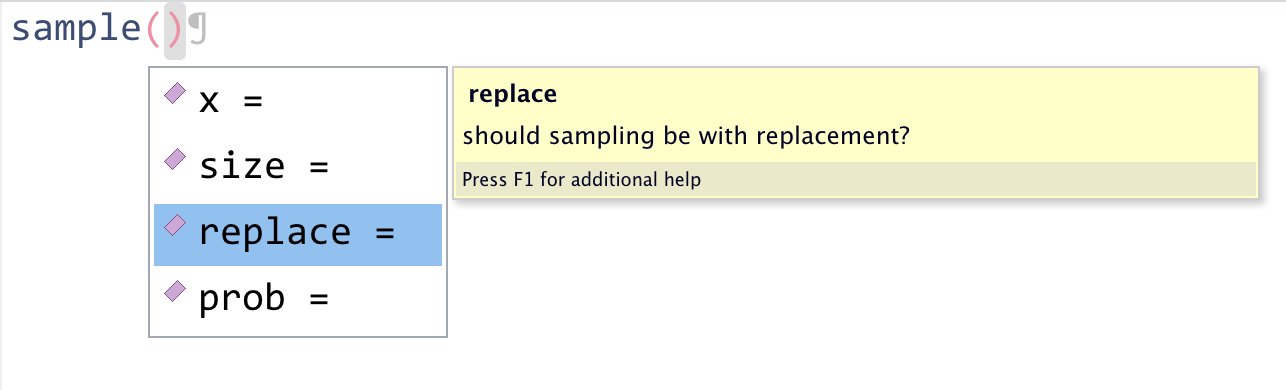
\includegraphics[width=1\linewidth]{images/intro/autocomplete} 

}

\caption{Tab auto-complete}\label{fig:img-autocomplete}
\end{figure}

\section{Objects}\label{objects}

A large part of your coding will involve creating and manipulating objects. Objects contain stuff. That stuff can be numbers, words, or the result of operations and analyses. You assign content to an object using \texttt{\textless{}-}.

Run the following code in the console, but change the values of \texttt{name} and \texttt{age} to your own details and change \texttt{christmas} to a holiday or date you care about.

\begin{Shaded}
\begin{Highlighting}[]
\NormalTok{name }\OtherTok{\textless{}{-}} \StringTok{"Emily"}
\NormalTok{age }\OtherTok{\textless{}{-}} \DecValTok{39}
\NormalTok{today }\OtherTok{\textless{}{-}} \FunctionTok{Sys.Date}\NormalTok{()}
\NormalTok{christmas }\OtherTok{\textless{}{-}} \FunctionTok{as.Date}\NormalTok{(}\StringTok{"2025{-}12{-}25"}\NormalTok{)}
\end{Highlighting}
\end{Shaded}

You'll see that four objects now appear in the environment pane:

\begin{itemize}
\tightlist
\item
  \texttt{name} is character{} (text) data. In order for R to recognise it as character data, it \textbf{must} be enclosed in double quotation marks \texttt{"\ "}.
\item
  \texttt{age} is numeric{} data. In order for R to recognise this as a number, it \textbf{must not} be enclosed in quotation marks.
\item
  \texttt{today} stores the result of the function \texttt{Sys.Date()}. This function returns your computer system's date. Unlike \texttt{name} and \texttt{age}, which are hard-coded (i.e., they will always return the values you enter), the contents of the object \texttt{today} will change dynamically with the date. That is, if you run that function tomorrow, it will update the date to tomorrow's date.
\item
  \texttt{christmas} is also a date but it's hard-coded as a very specific date. It's wrapped within the \texttt{as.Date()} function that tells R to interpret the character string you provide as date rather than text.
\end{itemize}

\begin{try}
To print the contents of an object, type the object's name in the console and press enter. Try printing all four objects now.

\end{try}

Finally, a key concept to understand is that objects can interact and you can save the results of those interactions in new object. Edit and run the following code to create these new objects, and then print the contents of each new object.

\begin{Shaded}
\begin{Highlighting}[]
\NormalTok{decade }\OtherTok{\textless{}{-}}\NormalTok{ age }\SpecialCharTok{+} \DecValTok{10}
\NormalTok{full\_name }\OtherTok{\textless{}{-}} \FunctionTok{paste}\NormalTok{(name, }\StringTok{"Nordmann"}\NormalTok{)}
\NormalTok{how\_long }\OtherTok{\textless{}{-}}\NormalTok{ christmas }\SpecialCharTok{{-}}\NormalTok{ today}
\end{Highlighting}
\end{Shaded}

\section{Getting help}\label{help}

You will feel like you need a \emph{lot} of help when you're starting to learn. This won't really go away; it's impossible to memorise everything. The goal is to learn enough about the structure of R that you can look things up quickly. This is why we'll introduce specialised jargon in the glossary; it's easier to google ``convert character{} to numeric{} in R'' than ``make numbers in quotes be actual numbers not words''. In addition to the function help described above, here's some additional resources you should use often.

\subsection{Package reference manuals}\label{package-reference-manuals}

Start up help in a browser by entering \texttt{help.start()} in the console. Click on ``Packages'' under ``Reference'' to see a list of packages. Scroll down to the \texttt{readxl} package and click on it to see a list of the functions that are available in that package.

\subsection{AI}\label{ai}

Large Language models are a fantastic resource to help you on your coding journey but you must use them criticially, and without strong foundations of core knowledge and skills, they can be very dangerous. We have written a companion book \href{https://psyteachr.github.io/AITutoR/}{AI TutoR} that takes you through how to use AI as a personal tutor and pair programmer.

\subsection{Googling}\label{googling}

If the function help doesn't help, or you're not even sure what function you need, try Googling your question. It will take some practice to be able to use the right jargon in your search terms to get what you want. It helps to put ``R'' or ``tidyverse'' in the search text, or the name of the relevant package, like ggplot2.

\subsection{Vignettes}\label{vignettes}

Many packages, especially \href{https://www.tidyverse.org/packages/}{tidyverse} ones, have helpful websites with vignettes explaining how to use their functions. Some of the vignettes are also available inside R. You can access them from a package's help page or with the \texttt{vignette()} function.

\begin{Shaded}
\begin{Highlighting}[]
\CommentTok{\# opens a list of available vignettes}
\FunctionTok{vignette}\NormalTok{(}\AttributeTok{package =} \StringTok{"ggplot2"}\NormalTok{)}

\CommentTok{\# opens a specific vignette in the Help pane}
\FunctionTok{vignette}\NormalTok{(}\StringTok{"ggplot2{-}specs"}\NormalTok{, }\AttributeTok{package =} \StringTok{"ggplot2"}\NormalTok{)}
\end{Highlighting}
\end{Shaded}

\section{Webinar set-up check}\label{workshop-prep}

Restart your R session and then run the below code by copying and pasting it all into the console and then hitting enter. If you have managed to install and update all software and packages as required, it should run without issue and produce the below histograms. It will produce some messages that look like errors involving \texttt{stat\_bin}, don't worry, they aren't errors and we'll explain what these messages mean in the workshop.

\begin{Shaded}
\begin{Highlighting}[]
\FunctionTok{library}\NormalTok{(tidyverse)}
\FunctionTok{library}\NormalTok{(patchwork)}
\FunctionTok{library}\NormalTok{(ggthemes)}

\FunctionTok{data}\NormalTok{(starwars)}

\NormalTok{mass }\OtherTok{\textless{}{-}} \FunctionTok{ggplot}\NormalTok{(starwars, }\FunctionTok{aes}\NormalTok{(}\AttributeTok{x =}\NormalTok{ mass)) }\SpecialCharTok{+}
  \FunctionTok{geom\_histogram}\NormalTok{() }\SpecialCharTok{+}
  \FunctionTok{theme\_economist}\NormalTok{() }\SpecialCharTok{+}
  \FunctionTok{labs}\NormalTok{(}\AttributeTok{title =} \StringTok{"Star Wars"}\NormalTok{, }
       \AttributeTok{subtitle =} \StringTok{"Character Mass (Kg)"}\NormalTok{,}
       \AttributeTok{x =} \ConstantTok{NULL}\NormalTok{, }\AttributeTok{y =} \ConstantTok{NULL}\NormalTok{)}

\NormalTok{height }\OtherTok{\textless{}{-}} \FunctionTok{ggplot}\NormalTok{(starwars, }\FunctionTok{aes}\NormalTok{(}\AttributeTok{x =}\NormalTok{ height)) }\SpecialCharTok{+}
  \FunctionTok{geom\_histogram}\NormalTok{() }\SpecialCharTok{+}
  \FunctionTok{theme\_economist}\NormalTok{() }\SpecialCharTok{+}
  \FunctionTok{labs}\NormalTok{(}\AttributeTok{subtitle =} \StringTok{"Character Height (cm)"}\NormalTok{,}
       \AttributeTok{x =} \ConstantTok{NULL}\NormalTok{, }\AttributeTok{y =} \ConstantTok{NULL}\NormalTok{)}

\NormalTok{mass }\SpecialCharTok{+}\NormalTok{ height}
\end{Highlighting}
\end{Shaded}

\begin{center}\includegraphics[width=1\linewidth]{01-intro-to-r_files/figure-latex/unnamed-chunk-6-1} \end{center}

If you get the error \texttt{there\ is\ no\ package\ called...}, make sure you have installed all the packages listed in Section~\ref{install-package}.

If you are having technical issues working on your own machine and cannot get the below code to run, please use \href{https://rstudio.cloud/}{RStudio Cloud} for the workshop as there will not be time to troubleshoot installation problems.

\section{Glossary}\label{glossary-intro}

\begin{table}
\centering
\begin{tabular}{l|l}
\hline
term & definition\\
\hline
argument & \\
\hline
base R & \\
\hline
character & \\
\hline
chunk & \\
\hline
conflict & \\
\hline
CRAN & \\
\hline
data wrangling & \\
\hline
factor & \\
\hline
function & \\
\hline
IDE & \\
\hline
knit & \\
\hline
numeric & \\
\hline
object & \\
\hline
package & \\
\hline
panes & \\
\hline
R Markdown & \\
\hline
reproducibility & \\
\hline
script & \\
\hline
string & \\
\hline
vector & \\
\hline
\end{tabular}
\end{table}

\section{Further Resources}\label{resources-intro}

\begin{itemize}
\tightlist
\item
  \href{https://raw.githubusercontent.com/rstudio/cheatsheets/main/rstudio-ide.pdf}{RStudio IDE Cheatsheet}
\item
  \href{https://rstudio.cloud/}{RStudio Cloud}
\end{itemize}

\chapter{Webinar}\label{webinar}

\section{Set-up}\label{set-up}

\begin{verbatim}
## Warning: package 'jtools' was built under R version 4.3.3
\end{verbatim}

\begin{verbatim}
## Warning: package 'ggExtra' was built under R version 4.3.3
\end{verbatim}

\begin{verbatim}
## Rows: 12570 Columns: 788
## -- Column specification --------------------------------------------------------
## Delimiter: ","
## chr (526): unique_id, survey_id, country, language, incentive, participation...
## dbl (247): progress, duration, Q7.1_1, Q7.1_2, Q7.1_3, Q7.1_4, Q7.1_5, Q7.1_...
## lgl  (15): topic_meta_analysis, in_person_seminars_specify, in_person_exam_s...
## 
## i Use `spec()` to retrieve the full column specification for this data.
## i Specify the column types or set `show_col_types = FALSE` to quiet this message.
\end{verbatim}

\begin{Shaded}
\begin{Highlighting}[]
\FunctionTok{library}\NormalTok{(tidyverse)}
\FunctionTok{library}\NormalTok{(jtools)}
\FunctionTok{library}\NormalTok{(ggExtra)}
\NormalTok{dat }\OtherTok{\textless{}{-}} \FunctionTok{read\_csv}\NormalTok{(}\StringTok{"smarvus\_complete\_050524.csv"}\NormalTok{)}
\end{Highlighting}
\end{Shaded}

The dataset is massive so we're going to look at just four different scales. This webinar doesn't have time to cover how to do this but if you're interested, the comments should tell you what it's doing (and you could ask AI to explain it to you as well).

This code creates four objects:

\begin{itemize}
\item
  demo has demographic information, age, gender, and degree major. Age data has been categorised for anonymisation purposes. The option `Implausible' describes values that were 99 or higher or 17 or lower.
\item
  STARS - Statistics anxiety was measured by the Statistics Anxiety Rating Scale (STARS; Cruise et al., 1985). Each item describes a situation involving statistics such as ``Doing an examination in a statistics course'' (test and class anxiety), ``Interpreting the meaning of a table in a journal article'' (interpretation anxiety), or ``Going to ask my statistics teacher for individual help with material I am having difficulty understanding'' (fear of asking for help).
\item
  BNFE - Fear of Negative Evaluation. Fear of negative evaluation was measured using the Brief Fear of Negative Evaluation Scale -- Straightforward (BNFE-S; Leary, 1983; Rodebaugh et al., 2004). The scale contains 8 items, including statements such as, ``I am afraid that people will find fault with me'' and ``I often worry that I will say or do the wrong things''.
\item
  IUS - Intolerance of Uncertainty. Intolerance of uncertainty was measured using the Intolerance of Uncertainty Scale -- Short Form (IUS-SF; Carleton et al., 2007). The scale contains 2 subscales, Prospective Anxiety and Inhibitory Anxiety, each with 6 items. The Prospective Anxiety subscale includes statements such as, ``The smallest doubt can stop me from acting''. The Inhibitory Anxiety subscale includes statements such as, ``It frustrates me not having all the information I need''.
\end{itemize}

For the three scales, the code takes the responses to each individual item and generates a single mean score for each participant.

\begin{Shaded}
\begin{Highlighting}[]
\NormalTok{demo }\OtherTok{\textless{}{-}}\NormalTok{ dat }\SpecialCharTok{\%\textgreater{}\%}
  \FunctionTok{select}\NormalTok{(unique\_id, age, gender, degree\_major)}

\NormalTok{STARS }\OtherTok{\textless{}{-}}\NormalTok{ dat }\SpecialCharTok{\%\textgreater{}\%}
  \FunctionTok{select}\NormalTok{(unique\_id, Q7}\FloatTok{.1}\NormalTok{\_1}\SpecialCharTok{:}\NormalTok{Q7}\FloatTok{.1}\NormalTok{\_24) }\SpecialCharTok{\%\textgreater{}\%} \CommentTok{\# select the STARS columns}
  \FunctionTok{filter}\NormalTok{(Q7}\FloatTok{.1}\NormalTok{\_24 }\SpecialCharTok{==} \DecValTok{1}\NormalTok{) }\SpecialCharTok{\%\textgreater{}\%} \CommentTok{\# remove those who failed the attention check}
  \FunctionTok{select}\NormalTok{(}\SpecialCharTok{{-}}\NormalTok{Q7}\FloatTok{.1}\NormalTok{\_24) }\SpecialCharTok{\%\textgreater{}\%} \CommentTok{\# remove the attention check column}
  \FunctionTok{pivot\_longer}\NormalTok{(}\AttributeTok{cols =}\NormalTok{ Q7}\FloatTok{.1}\NormalTok{\_1}\SpecialCharTok{:}\NormalTok{Q7}\FloatTok{.1}\NormalTok{\_23, }\AttributeTok{names\_to =} \StringTok{"item"}\NormalTok{, }\AttributeTok{values\_to =} \StringTok{"score"}\NormalTok{) }\SpecialCharTok{\%\textgreater{}\%} \CommentTok{\# transform to long{-}form}
  \FunctionTok{group\_by}\NormalTok{(unique\_id) }\SpecialCharTok{\%\textgreater{}\%} \CommentTok{\# group by participant}
  \FunctionTok{summarise}\NormalTok{(}\AttributeTok{stars\_score =} \FunctionTok{mean}\NormalTok{(score, }\AttributeTok{na.rm =} \ConstantTok{TRUE}\NormalTok{)) }\SpecialCharTok{\%\textgreater{}\%} \CommentTok{\# calculate mean STARS score for each ppt}
  \FunctionTok{ungroup}\NormalTok{() }\SpecialCharTok{\%\textgreater{}\%} \CommentTok{\# ungroup so it doesn\textquotesingle{}t mess things up later}
  \FunctionTok{drop\_na}\NormalTok{() }\CommentTok{\#  get rid of NAs so they don\textquotesingle{}t cause us havoc}

\CommentTok{\# Brief Fear of Negative Evaluation Scale}

\NormalTok{BNFE }\OtherTok{\textless{}{-}}\NormalTok{ dat }\SpecialCharTok{\%\textgreater{}\%}
  \FunctionTok{select}\NormalTok{(unique\_id, Q11}\FloatTok{.1}\NormalTok{\_1}\SpecialCharTok{:}\NormalTok{Q11}\FloatTok{.1}\NormalTok{\_9) }\SpecialCharTok{\%\textgreater{}\%} \CommentTok{\# select the BNFE columns}
  \FunctionTok{filter}\NormalTok{(Q11}\FloatTok{.1}\NormalTok{\_9 }\SpecialCharTok{==} \DecValTok{3}\NormalTok{) }\SpecialCharTok{\%\textgreater{}\%} \CommentTok{\# remove those who failed the attention check}
  \FunctionTok{select}\NormalTok{(}\SpecialCharTok{{-}}\NormalTok{Q11}\FloatTok{.1}\NormalTok{\_9) }\SpecialCharTok{\%\textgreater{}\%} \CommentTok{\# remove the attention check column}
  \FunctionTok{pivot\_longer}\NormalTok{(}\AttributeTok{cols =}\NormalTok{ Q11}\FloatTok{.1}\NormalTok{\_1}\SpecialCharTok{:}\NormalTok{Q11}\FloatTok{.1}\NormalTok{\_8, }\AttributeTok{names\_to =} \StringTok{"item"}\NormalTok{, }\AttributeTok{values\_to =} \StringTok{"score"}\NormalTok{) }\SpecialCharTok{\%\textgreater{}\%} \CommentTok{\# transform to long{-}form}
  \FunctionTok{group\_by}\NormalTok{(unique\_id) }\SpecialCharTok{\%\textgreater{}\%} \CommentTok{\# group by participant}
  \FunctionTok{summarise}\NormalTok{(}\AttributeTok{bnfe\_score =} \FunctionTok{mean}\NormalTok{(score, }\AttributeTok{na.rm =} \ConstantTok{TRUE}\NormalTok{)) }\SpecialCharTok{\%\textgreater{}\%} \CommentTok{\# calculate mean BNFE score for each ppt}
  \FunctionTok{ungroup}\NormalTok{() }\SpecialCharTok{\%\textgreater{}\%} \CommentTok{\# ungroup so it doesn\textquotesingle{}t mess things up later}
  \FunctionTok{drop\_na}\NormalTok{() }\CommentTok{\#  get rid of NAs so they don\textquotesingle{}t cause us havoc}

\CommentTok{\# Intolerance of Uncertainty.}

\NormalTok{IUS }\OtherTok{\textless{}{-}}\NormalTok{ dat }\SpecialCharTok{\%\textgreater{}\%}
  \FunctionTok{select}\NormalTok{(unique\_id, Q14}\FloatTok{.1}\NormalTok{\_1}\SpecialCharTok{:}\NormalTok{Q14}\FloatTok{.1}\NormalTok{\_12) }\SpecialCharTok{\%\textgreater{}\%} \CommentTok{\# select the BNFE columns}
  \FunctionTok{pivot\_longer}\NormalTok{(}\AttributeTok{cols =}\NormalTok{ Q14}\FloatTok{.1}\NormalTok{\_1}\SpecialCharTok{:}\NormalTok{Q14}\FloatTok{.1}\NormalTok{\_12, }\AttributeTok{names\_to =} \StringTok{"item"}\NormalTok{, }\AttributeTok{values\_to =} \StringTok{"score"}\NormalTok{) }\SpecialCharTok{\%\textgreater{}\%} \CommentTok{\# transform to long{-}form}
  \FunctionTok{group\_by}\NormalTok{(unique\_id) }\SpecialCharTok{\%\textgreater{}\%} \CommentTok{\# group by participant}
  \FunctionTok{summarise}\NormalTok{(}\AttributeTok{ius\_score =} \FunctionTok{mean}\NormalTok{(score, }\AttributeTok{na.rm =} \ConstantTok{TRUE}\NormalTok{)) }\SpecialCharTok{\%\textgreater{}\%} \CommentTok{\# calculate mean IUS{-}SF score for each ppt}
  \FunctionTok{ungroup}\NormalTok{() }\SpecialCharTok{\%\textgreater{}\%} \CommentTok{\# ungroup so it doesn\textquotesingle{}t mess things up later}
  \FunctionTok{drop\_na}\NormalTok{() }\CommentTok{\#  get rid of NAs so they don\textquotesingle{}t cause us havoc}

\CommentTok{\# join everything together}

\NormalTok{dat\_joined }\OtherTok{\textless{}{-}} \FunctionTok{inner\_join}\NormalTok{(}\AttributeTok{x =}\NormalTok{ demo, }\AttributeTok{y =}\NormalTok{ STARS, }\AttributeTok{by =} \StringTok{"unique\_id"}\NormalTok{) }\SpecialCharTok{\%\textgreater{}\%}
  \FunctionTok{inner\_join}\NormalTok{(BNFE, }\AttributeTok{by =} \StringTok{"unique\_id"}\NormalTok{) }\SpecialCharTok{\%\textgreater{}\%}
  \FunctionTok{inner\_join}\NormalTok{(IUS, }\AttributeTok{by =} \StringTok{"unique\_id"}\NormalTok{)}

\CommentTok{\# convert categorical data to factors}

\NormalTok{dat\_joined }\OtherTok{\textless{}{-}}\NormalTok{ dat\_joined }\SpecialCharTok{\%\textgreater{}\%}
  \FunctionTok{mutate}\NormalTok{(}\AttributeTok{age =} \FunctionTok{as.factor}\NormalTok{(age),}
         \AttributeTok{gender =} \FunctionTok{as.factor}\NormalTok{(gender),}
         \AttributeTok{degree\_major =} \FunctionTok{as.factor}\NormalTok{(degree\_major))}

\CommentTok{\# take a subset of the data because some groups have very small sample sizes}

\NormalTok{dat\_final }\OtherTok{\textless{}{-}}\NormalTok{ dat\_joined }\SpecialCharTok{\%\textgreater{}\%}
  \FunctionTok{filter}\NormalTok{(gender }\SpecialCharTok{\%in\%} \FunctionTok{c}\NormalTok{(}\StringTok{"Female/Woman"}\NormalTok{, }\StringTok{"Male/Man"}\NormalTok{)) }\SpecialCharTok{\%\textgreater{}\%}
  \FunctionTok{mutate}\NormalTok{(}\AttributeTok{age =} \FunctionTok{case\_when}\NormalTok{(age }\SpecialCharTok{==} \StringTok{"18{-}21"} \SpecialCharTok{\textasciitilde{}} \StringTok{"18{-}21"}\NormalTok{,}
\NormalTok{                         age }\SpecialCharTok{==} \StringTok{"22{-}25"} \SpecialCharTok{\textasciitilde{}} \StringTok{"22+"}\NormalTok{,}
\NormalTok{                         age }\SpecialCharTok{==} \StringTok{"26+"} \SpecialCharTok{\textasciitilde{}} \StringTok{"22+"}\NormalTok{)) }\SpecialCharTok{\%\textgreater{}\%}
  \FunctionTok{drop\_na}\NormalTok{(age)}

\CommentTok{\# remove all the objects we don\textquotesingle{}t need }

\FunctionTok{rm}\NormalTok{(}\AttributeTok{list =} \FunctionTok{c}\NormalTok{(}\StringTok{"BNFE"}\NormalTok{, }\StringTok{"dat"}\NormalTok{, }\StringTok{"dat\_joined"}\NormalTok{, }\StringTok{"demo"}\NormalTok{, }\StringTok{"IUS"}\NormalTok{, }\StringTok{"STARS"}\NormalTok{))}
\end{Highlighting}
\end{Shaded}

\section{The Grammar of Graphics}\label{the-grammar-of-graphics}

The \texttt{ggplot2} package is based on \textbf{the Grammar of Graphics}, a theoretical framework developed by Leland Wilkinson (2005), which describes how statistical graphics are constructed from a layered and modular set of components. This approach treats graphics as a visual language, where each plot is built by combining several independent elements such as data, mappings (aesthetic relationships between data and visual properties), geometric objects, statistical transformations, coordinate systems, and themes.

At its core, \texttt{ggplot2} requires at least three elements:
1. \textbf{A dataset}, containing the variables of interest.
2. \textbf{Aesthetics (\texttt{aes()})}, which map variables in the dataset to visual properties such as position, colour, size, and shape.
3. \textbf{Geometric objects (\texttt{geoms})}, which specify what kind of plot to draw---e.g., bars, points, lines, or boxplots.

Together, these components form a flexible system that allows users to build complex and meaningful data visualisations in a structured way. For example:

This modular design encourages users to think critically about the story they want their data to tell and to construct visualisations that are both analytically rigorous and aesthetically effective (Healy, 2018). It also facilitates reproducibility and clarity in data science workflows, as each component of the plot is explicitly stated in the code.

\begin{Shaded}
\begin{Highlighting}[]
\CommentTok{\# the base}
\FunctionTok{ggplot}\NormalTok{()}
\end{Highlighting}
\end{Shaded}

\begin{center}
\includegraphics[width=1\linewidth]{02-webinar_files/figure-latex/unnamed-chunk-4-1} \end{center}

\begin{Shaded}
\begin{Highlighting}[]
\CommentTok{\# adding in data set}
\FunctionTok{ggplot}\NormalTok{(}\AttributeTok{data =}\NormalTok{ dat\_final, }\FunctionTok{aes}\NormalTok{(}\AttributeTok{x =}\NormalTok{ stars\_score))}
\end{Highlighting}
\end{Shaded}

\begin{center}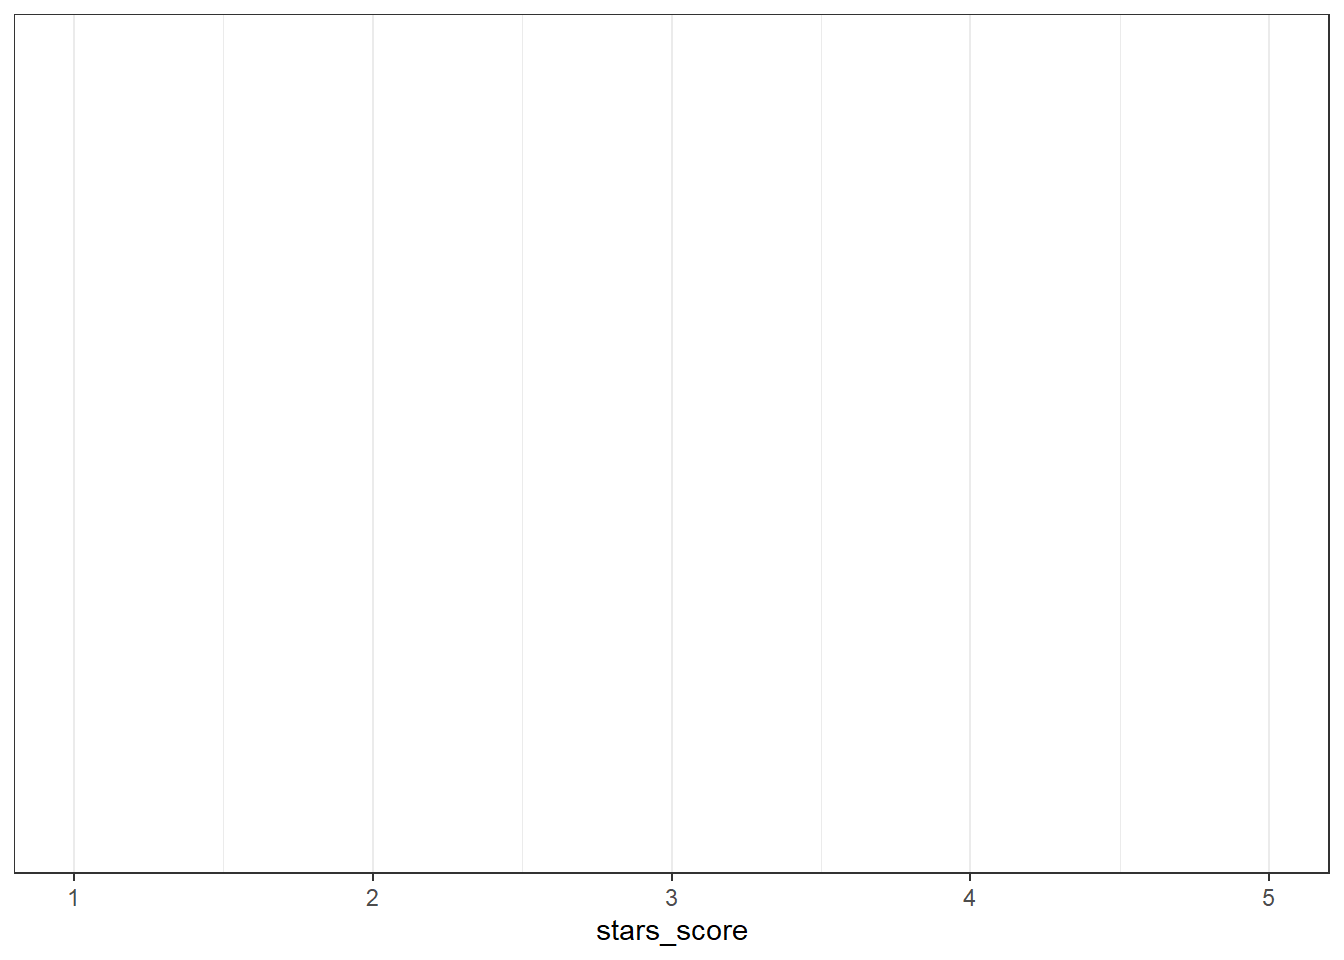
\includegraphics[width=1\linewidth]{02-webinar_files/figure-latex/unnamed-chunk-4-2} \end{center}

\begin{Shaded}
\begin{Highlighting}[]
\CommentTok{\# adding layers}
\FunctionTok{ggplot}\NormalTok{(}\AttributeTok{data =}\NormalTok{ dat\_final, }\FunctionTok{aes}\NormalTok{(}\AttributeTok{x =}\NormalTok{ stars\_score)) }\SpecialCharTok{+}
  \FunctionTok{geom\_histogram}\NormalTok{()}
\end{Highlighting}
\end{Shaded}

\begin{verbatim}
## `stat_bin()` using `bins = 30`. Pick better value with `binwidth`.
\end{verbatim}

\begin{center}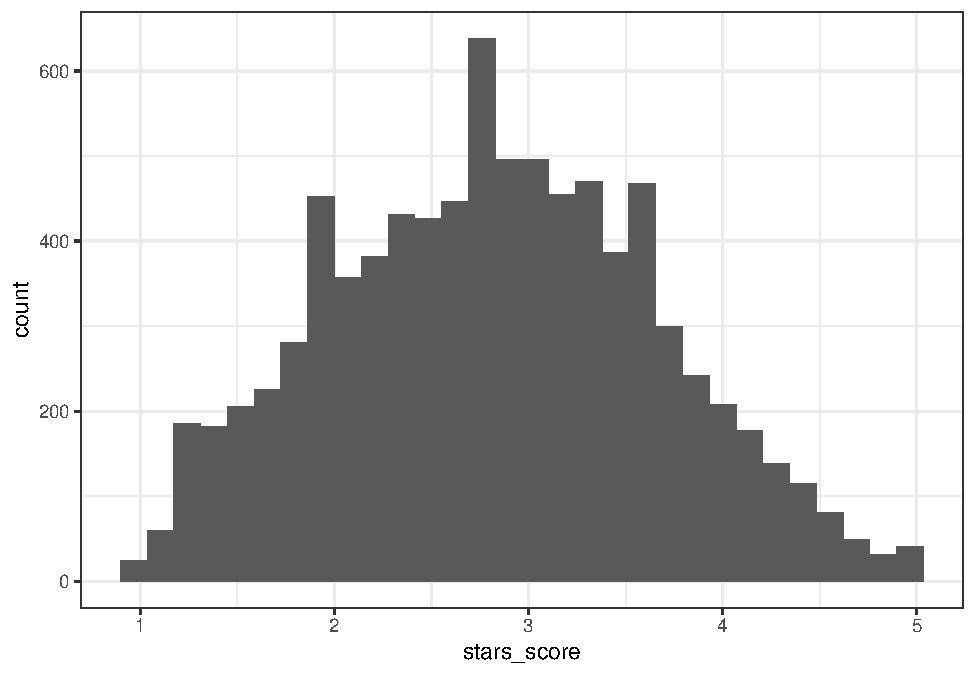
\includegraphics[width=1\linewidth]{02-webinar_files/figure-latex/unnamed-chunk-4-3} \end{center}

\begin{Shaded}
\begin{Highlighting}[]
\CommentTok{\# adding more layers}
\FunctionTok{ggplot}\NormalTok{(}\AttributeTok{data =}\NormalTok{ dat\_final, }\FunctionTok{aes}\NormalTok{(stars\_score)) }\SpecialCharTok{+}
  \FunctionTok{geom\_histogram}\NormalTok{() }\SpecialCharTok{+}
  \FunctionTok{labs}\NormalTok{(}\AttributeTok{title =} \StringTok{"My first histogram"}\NormalTok{,}
       \AttributeTok{x =} \StringTok{"Mean STARS score"}\NormalTok{,}
       \AttributeTok{caption =} \StringTok{"Isn\textquotesingle{}t R fun"}\NormalTok{)}
\end{Highlighting}
\end{Shaded}

\begin{verbatim}
## `stat_bin()` using `bins = 30`. Pick better value with `binwidth`.
\end{verbatim}

\begin{center}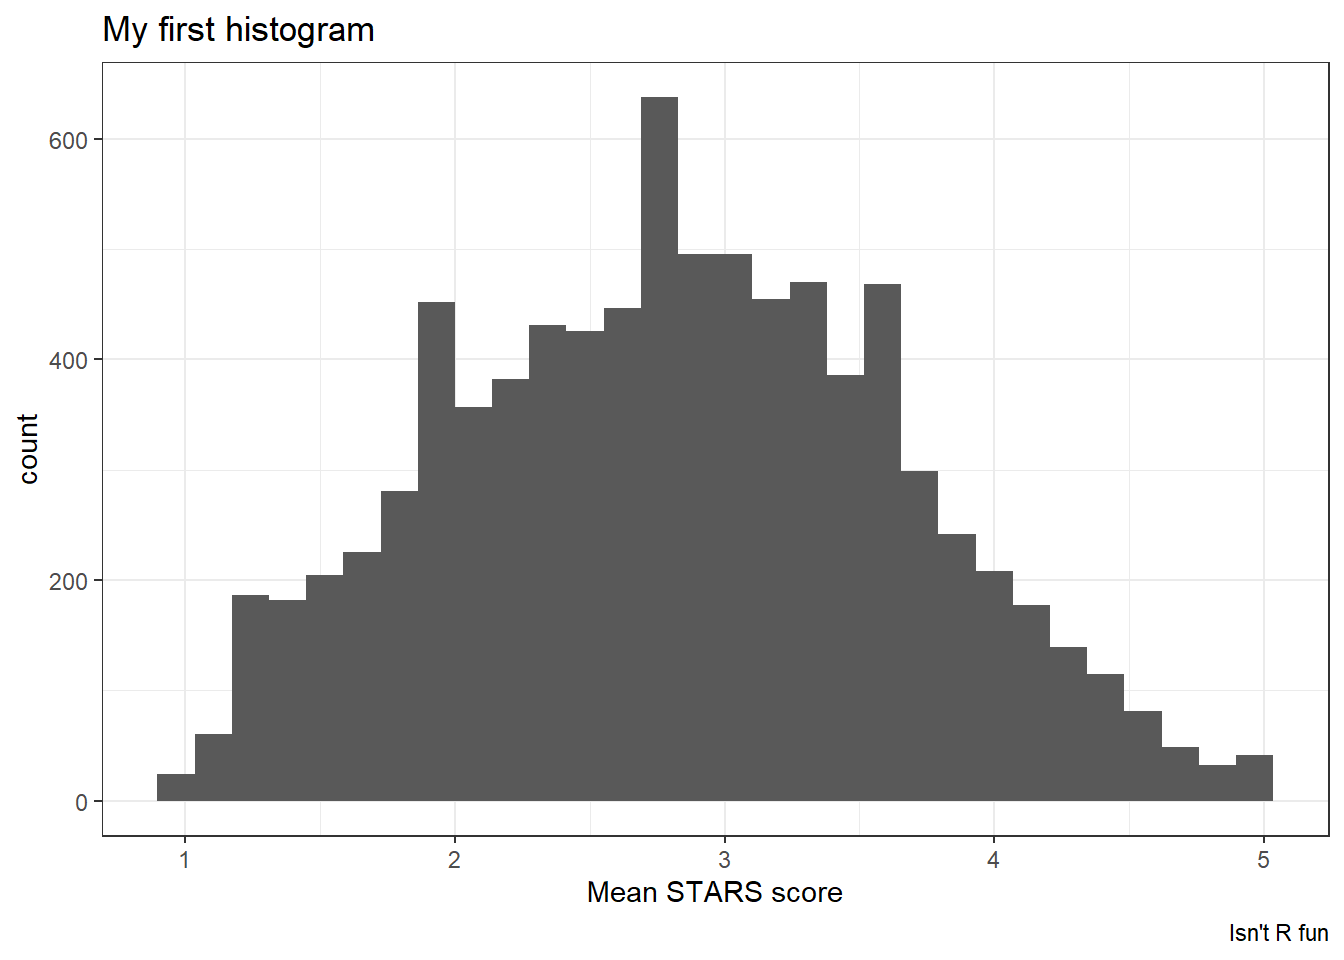
\includegraphics[width=1\linewidth]{02-webinar_files/figure-latex/unnamed-chunk-4-4} \end{center}

\section{Plot types}\label{plot-types}

\subsection{One categorical variable}\label{one-categorical-variable}

When you have a single \textbf{categorical variable}, a \textbf{bar chart} is typically the most appropriate way to visualise the frequency (i.e., count) of each category. In \texttt{ggplot2}, this is achieved using \texttt{geom\_bar()}, which by default \textbf{counts the number of observations} in each category and plots those counts as bars.

\subsubsection{Important note:}\label{important-note}

\texttt{geom\_bar()} should not be confused with \texttt{geom\_col()}. While \texttt{geom\_bar()} \textbf{calculates the y-values (counts) automatically}, \texttt{geom\_col()} requires you to \textbf{supply both x and y values explicitly}, and is typically used when you are plotting summary statistics (e.g., means, proportions).

\subsubsection{Why we do not plot means for a single categorical variable:}\label{why-we-do-not-plot-means-for-a-single-categorical-variable}

A common mistake is to try to use a bar chart to visualise the \textbf{mean of a numeric variable} for each category. This approach is often discouraged because bar heights suggest frequencies, and the lack of distributional information (e.g., variability or sample size) can be misleading. Instead, when you wish to compare a numeric outcome across groups, better options include:
- \textbf{Boxplots}: Show medians, quartiles, and potential outliers.
- \textbf{Violin plots}: Combine density estimation with summary statistics.
- \textbf{Dotplots or jittered points}: Especially helpful when sample sizes are small.

That said, for purely categorical data---such as visualising how many students are enrolled in each degree programme or how many participants identify with a particular gender---bar charts are both simple and effective.

\begin{Shaded}
\begin{Highlighting}[]
\FunctionTok{ggplot}\NormalTok{(dat\_final, }\FunctionTok{aes}\NormalTok{(}\AttributeTok{x =}\NormalTok{ degree\_major)) }\SpecialCharTok{+}
  \FunctionTok{geom\_bar}\NormalTok{()}
\end{Highlighting}
\end{Shaded}

\begin{center}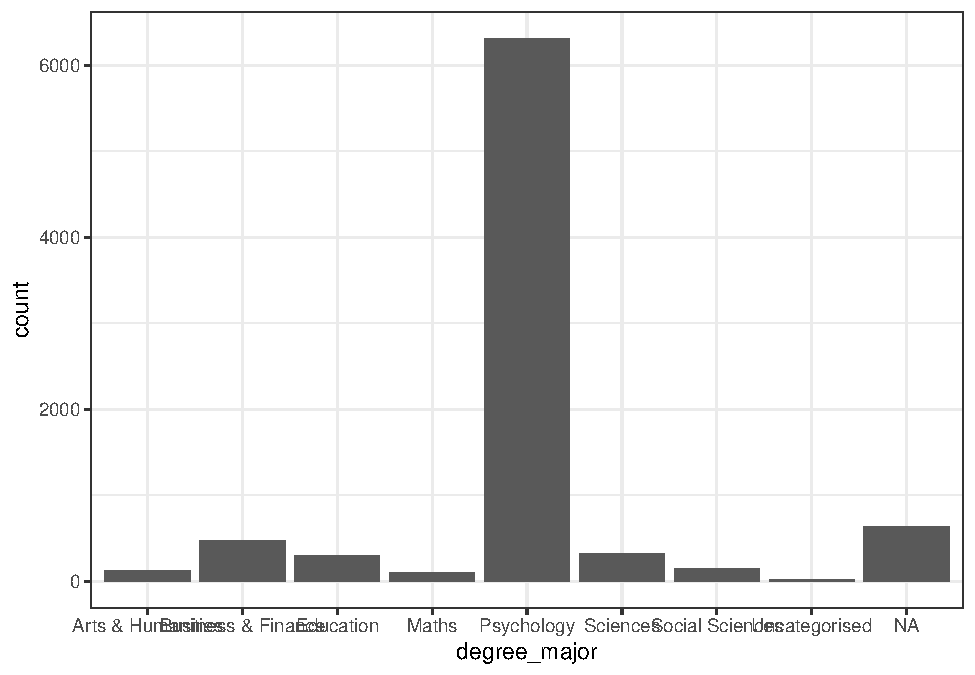
\includegraphics[width=1\linewidth]{02-webinar_files/figure-latex/unnamed-chunk-5-1} \end{center}

\subsection{One continuous variable}\label{one-continuous-variable}

When you have a single \textbf{continuous variable}, one of the most informative and commonly used visualisations is the \textbf{histogram}. Histograms show the \textbf{distribution} of a continuous variable by dividing the range of values into \textbf{intervals}, known as \emph{bins}, and then counting how many observations fall into each bin. The resulting bars provide a visual summary of the \textbf{shape, centre, and spread} of the data.

\subsubsection{Considerations when choosing bin width}\label{considerations-when-choosing-bin-width}

The choice of bin width is crucial. A \textbf{bin width that is too large} can obscure important features of the distribution, such as multimodality or skewness. Conversely, a \textbf{bin width that is too small} may introduce too much noise, creating a fragmented plot that is difficult to interpret.

Histograms are best suited for \textbf{exploratory data analysis}, allowing researchers to assess:
- Whether the distribution is symmetric, skewed, or multimodal,
- The presence of outliers or gaps,
- The approximate range and density of values.

As a visualisation of a single variable, histograms serve as a critical first step in understanding the structure of your data.

\begin{Shaded}
\begin{Highlighting}[]
\FunctionTok{ggplot}\NormalTok{(}\AttributeTok{data =}\NormalTok{ dat\_final, }\FunctionTok{aes}\NormalTok{(stars\_score)) }\SpecialCharTok{+}
  \FunctionTok{geom\_histogram}\NormalTok{(}\AttributeTok{binwidth =}\NormalTok{ .}\DecValTok{25}\NormalTok{, }
                 \AttributeTok{boundary =} \DecValTok{0}\NormalTok{, }
                 \AttributeTok{colour =} \StringTok{"black"}\NormalTok{,}
                 \AttributeTok{fill =} \StringTok{"lightblue"}\NormalTok{) }
\end{Highlighting}
\end{Shaded}

\begin{center}\includegraphics[width=1\linewidth]{02-webinar_files/figure-latex/unnamed-chunk-6-1} \end{center}

\subsection{One Continuous, One Categorical Variable}\label{one-continuous-one-categorical-variable}

When visualising the relationship between a \textbf{continuous variable} and a \textbf{categorical variable}, the goal is typically to compare the \textbf{distribution of the continuous variable across the levels of the categorical variable}. Several types of plots can be used for this purpose, each offering different advantages depending on the nature of the data and the story one wishes to tell.

One of the most common and informative options is the \textbf{boxplot}. A boxplot provides a compact summary of the distribution of the continuous variable within each category. It shows the median, interquartile range, and potential outliers, allowing for quick visual comparisons of central tendency and spread between groups. Boxplots are particularly useful when comparing several groups side by side, as they are less sensitive to skewness and extreme values than some other visualisations.

An alternative is the \textbf{violin plot}, which builds upon the boxplot by incorporating a mirrored density plot on each side of the box. This adds information about the shape of the distribution, including multimodality, while still retaining the median and interquartile range. Violin plots are well suited to larger datasets, where the estimation of the density is more stable.

Another option is the \textbf{histogram stratified by group}. This can be implemented in one of several ways:
- By overlaying histograms using colour or transparency,
- By ``dodging'' the bars to place them side by side, or
- By using faceting to produce a separate plot for each group.

Each of these approaches has trade-offs. Overlaid histograms can obscure the data if the number of groups is large or if the distributions overlap substantially. Dodged histograms make group comparisons easier but may misrepresent frequency when bins align differently between groups. Faceting, where each group is displayed in a separate panel, provides the clearest visual separation but makes direct comparisons slightly more difficult unless axes are held constant.

Finally, \textbf{density plots} serve a similar purpose to histograms but offer a smooth, continuous estimate of the distribution. When stratified by a categorical variable, density plots are effective for assessing overlap, skewness, and differences in modality between groups. However, unlike histograms, density plots do not represent actual counts or frequencies, and their interpretation may be less intuitive for novice audiences.

In choosing among these options, one should consider the \textbf{sample size}, the \textbf{shape and variability of the data}, and the \textbf{intended audience}. For smaller samples, more granular plots such as jittered points or dot plots may be more appropriate. For larger samples, density-based methods and summaries such as boxplots or violins become more effective.

Understanding how to visualise a continuous variable across groups is fundamental for comparing subpopulations, evaluating treatment effects, or identifying systematic differences in observational data.

\subsubsection{Grouped histograms}\label{grouped-histograms}

\begin{Shaded}
\begin{Highlighting}[]
\CommentTok{\# grouped by colour}
\FunctionTok{ggplot}\NormalTok{(dat\_final, }\FunctionTok{aes}\NormalTok{(}\AttributeTok{x =}\NormalTok{ stars\_score, }\AttributeTok{fill =}\NormalTok{ gender)) }\SpecialCharTok{+}
  \FunctionTok{geom\_histogram}\NormalTok{(}\AttributeTok{binwidth =}\NormalTok{ .}\DecValTok{25}\NormalTok{, }
                 \AttributeTok{boundary =} \DecValTok{0}\NormalTok{)}
\end{Highlighting}
\end{Shaded}

\begin{center}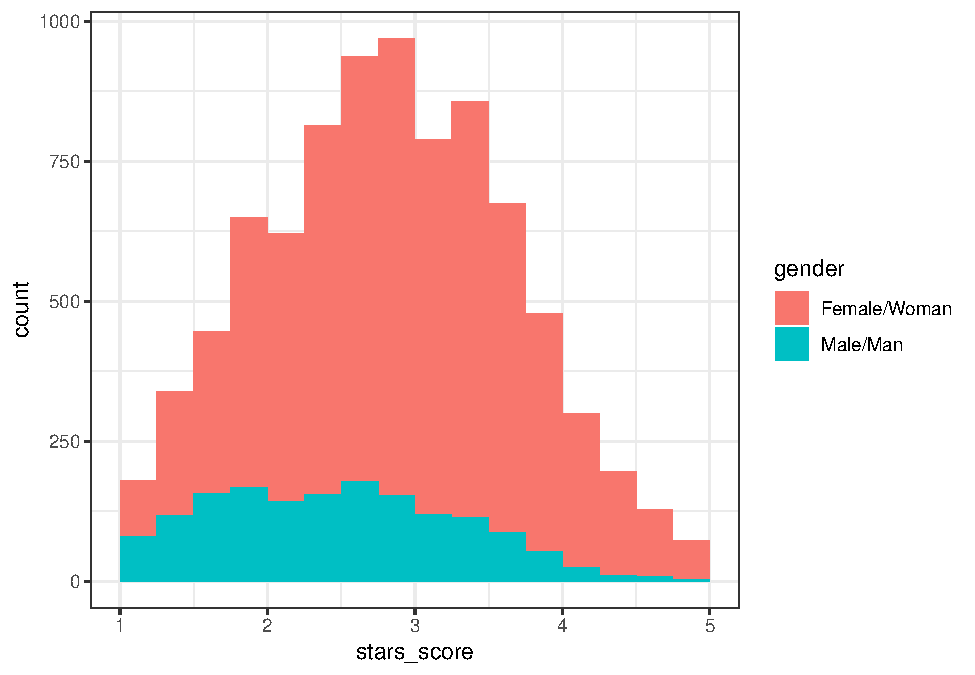
\includegraphics[width=1\linewidth]{02-webinar_files/figure-latex/unnamed-chunk-7-1} \end{center}

\begin{Shaded}
\begin{Highlighting}[]
\CommentTok{\# dodged bars}
\FunctionTok{ggplot}\NormalTok{(dat\_final, }\FunctionTok{aes}\NormalTok{(}\AttributeTok{x =}\NormalTok{ stars\_score, }\AttributeTok{fill =}\NormalTok{ gender)) }\SpecialCharTok{+}
  \FunctionTok{geom\_histogram}\NormalTok{(}\AttributeTok{binwidth =}\NormalTok{ .}\DecValTok{25}\NormalTok{, }
                 \AttributeTok{boundary =} \DecValTok{0}\NormalTok{,}
                 \AttributeTok{position =} \StringTok{"dodge"}\NormalTok{)}
\end{Highlighting}
\end{Shaded}

\begin{center}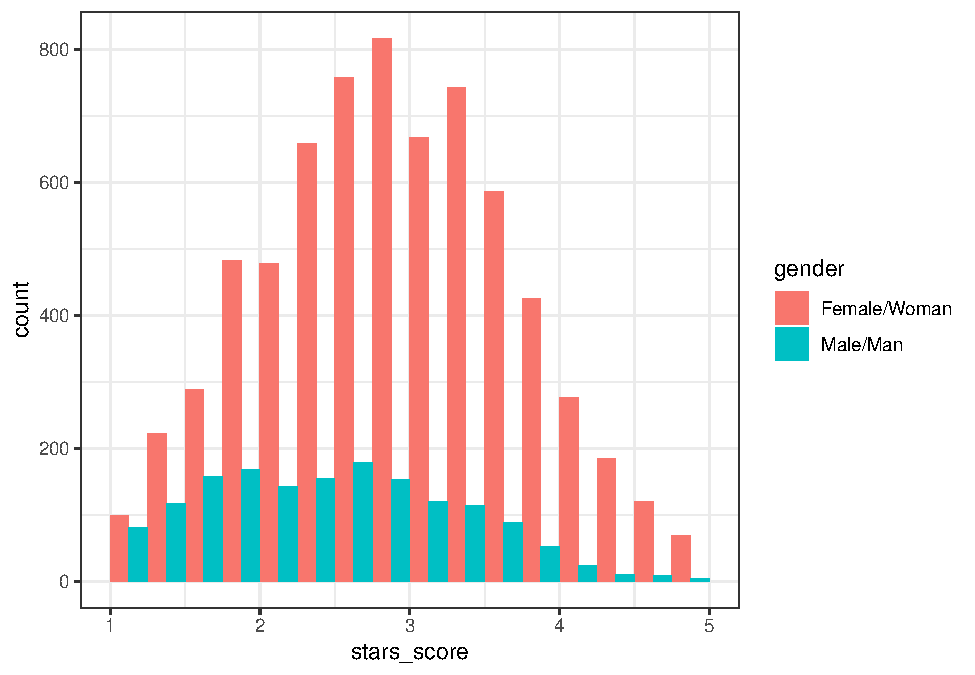
\includegraphics[width=1\linewidth]{02-webinar_files/figure-latex/unnamed-chunk-7-2} \end{center}

\begin{Shaded}
\begin{Highlighting}[]
\CommentTok{\# faceted histogram}
\FunctionTok{ggplot}\NormalTok{(dat\_final, }\FunctionTok{aes}\NormalTok{(}\AttributeTok{x =}\NormalTok{ stars\_score)) }\SpecialCharTok{+}
  \FunctionTok{geom\_histogram}\NormalTok{(}\AttributeTok{binwidth =}\NormalTok{ .}\DecValTok{25}\NormalTok{, }
                 \AttributeTok{boundary =} \DecValTok{0}\NormalTok{) }\SpecialCharTok{+}
  \FunctionTok{facet\_wrap}\NormalTok{(}\SpecialCharTok{\textasciitilde{}}\NormalTok{gender, }\AttributeTok{nrow =} \DecValTok{2}\NormalTok{, }\AttributeTok{scales =} \StringTok{"free\_y"}\NormalTok{)}
\end{Highlighting}
\end{Shaded}

\begin{center}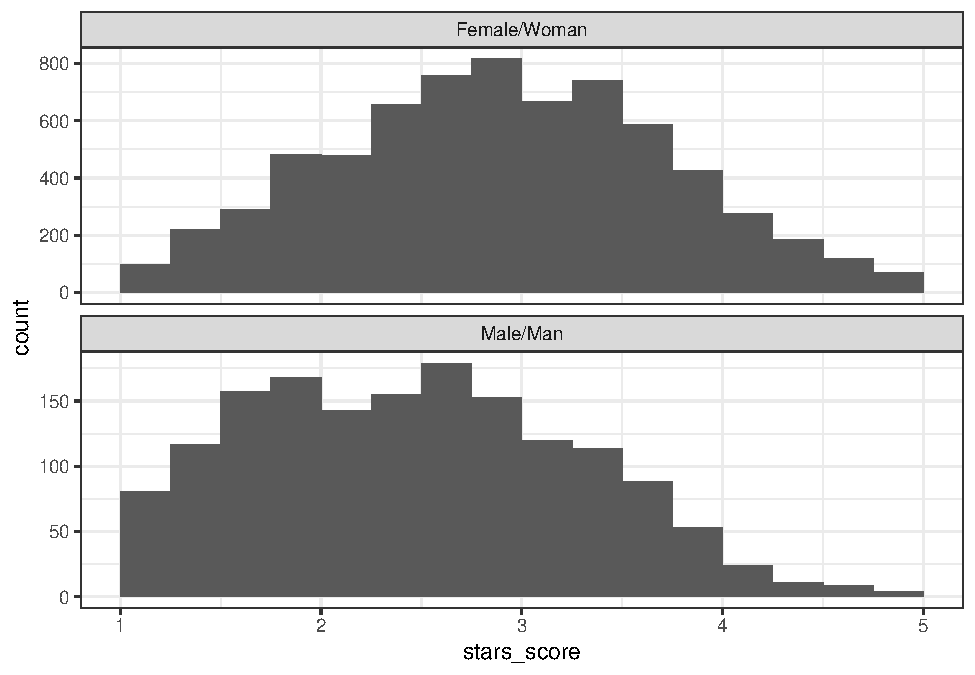
\includegraphics[width=1\linewidth]{02-webinar_files/figure-latex/unnamed-chunk-7-3} \end{center}

\subsubsection{Density plots}\label{density-plots}

\begin{Shaded}
\begin{Highlighting}[]
\FunctionTok{ggplot}\NormalTok{(}\AttributeTok{data =}\NormalTok{ dat\_final, }\FunctionTok{aes}\NormalTok{(}\AttributeTok{x =}\NormalTok{ stars\_score, }\AttributeTok{fill =}\NormalTok{ gender)) }\SpecialCharTok{+}
  \FunctionTok{geom\_density}\NormalTok{(}\AttributeTok{alpha =}\NormalTok{ .}\DecValTok{4}\NormalTok{)}
\end{Highlighting}
\end{Shaded}

\begin{center}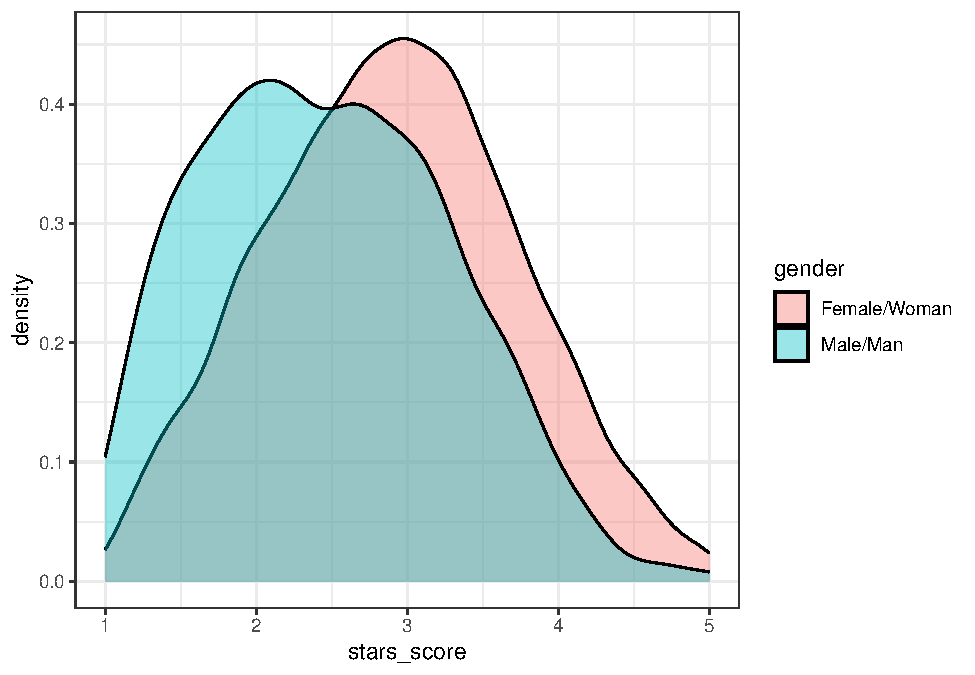
\includegraphics[width=1\linewidth]{02-webinar_files/figure-latex/unnamed-chunk-8-1} \end{center}

\subsubsection{Boxplots}\label{boxplots}

\begin{Shaded}
\begin{Highlighting}[]
\FunctionTok{ggplot}\NormalTok{(dat\_final, }\FunctionTok{aes}\NormalTok{(}\AttributeTok{x =}\NormalTok{ gender, }\AttributeTok{y =}\NormalTok{ stars\_score)) }\SpecialCharTok{+}
  \FunctionTok{geom\_boxplot}\NormalTok{()}
\end{Highlighting}
\end{Shaded}

\begin{center}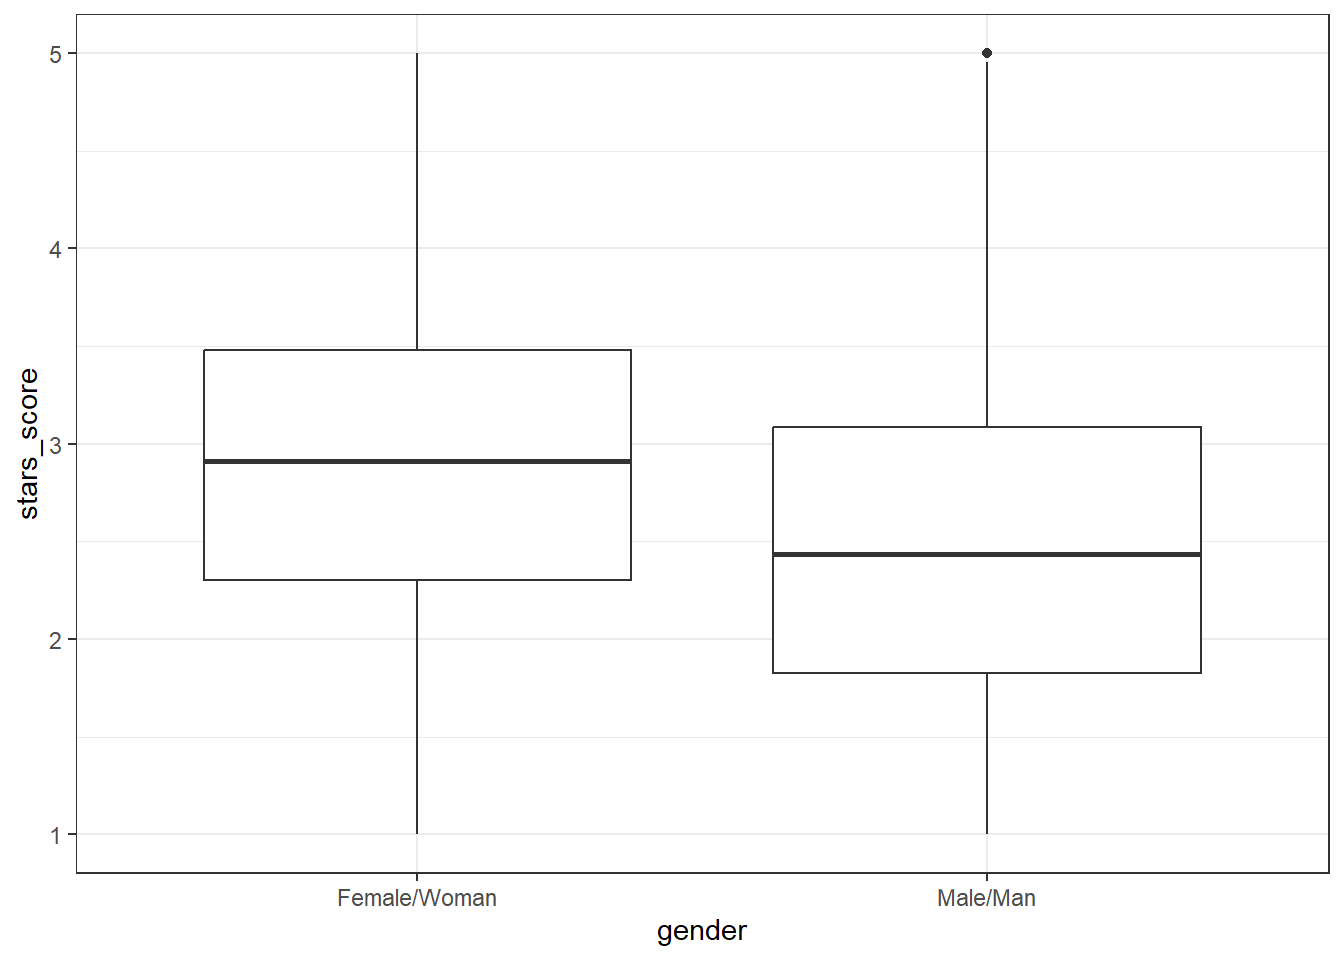
\includegraphics[width=1\linewidth]{02-webinar_files/figure-latex/unnamed-chunk-9-1} \end{center}

\subsubsection{Violin plots}\label{violin-plots}

\begin{Shaded}
\begin{Highlighting}[]
\FunctionTok{ggplot}\NormalTok{(dat\_final, }\FunctionTok{aes}\NormalTok{(}\AttributeTok{x =}\NormalTok{ gender, }\AttributeTok{y =}\NormalTok{ stars\_score)) }\SpecialCharTok{+}
  \FunctionTok{geom\_violin}\NormalTok{()}
\end{Highlighting}
\end{Shaded}

\begin{center}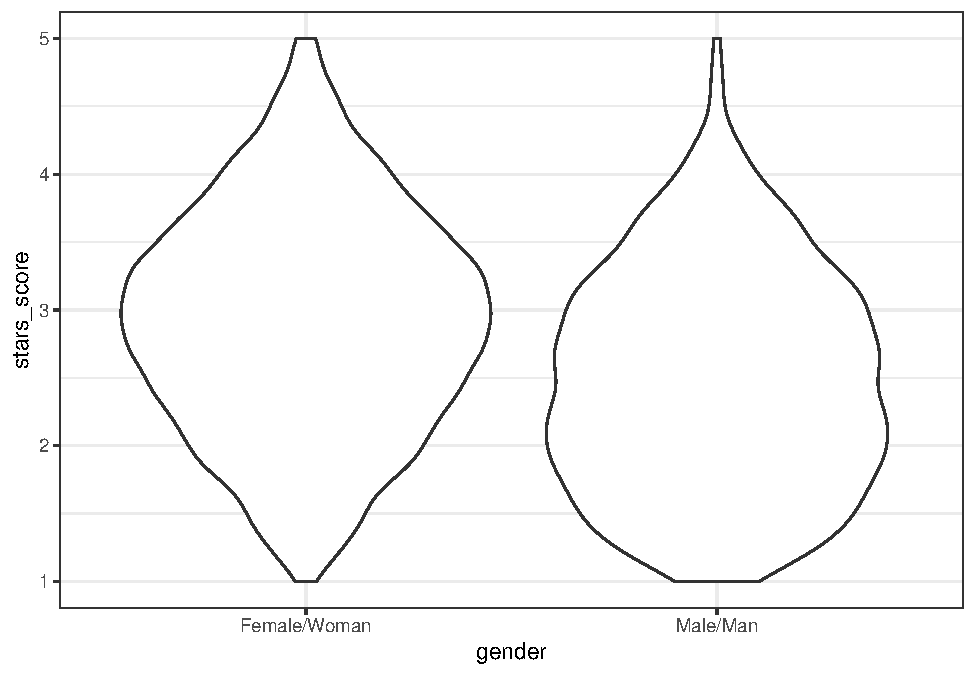
\includegraphics[width=1\linewidth]{02-webinar_files/figure-latex/unnamed-chunk-10-1} \end{center}

\subsubsection{Violin-boxplots}\label{violin-boxplots}

The order of layers matters!

\begin{Shaded}
\begin{Highlighting}[]
\FunctionTok{ggplot}\NormalTok{(dat\_final, }\FunctionTok{aes}\NormalTok{(}\AttributeTok{x =}\NormalTok{ gender, }\AttributeTok{y =}\NormalTok{ stars\_score)) }\SpecialCharTok{+}
  \FunctionTok{geom\_violin}\NormalTok{() }\SpecialCharTok{+}
  \FunctionTok{geom\_boxplot}\NormalTok{(}\AttributeTok{width =}\NormalTok{ .}\DecValTok{2}\NormalTok{)}
\end{Highlighting}
\end{Shaded}

\begin{center}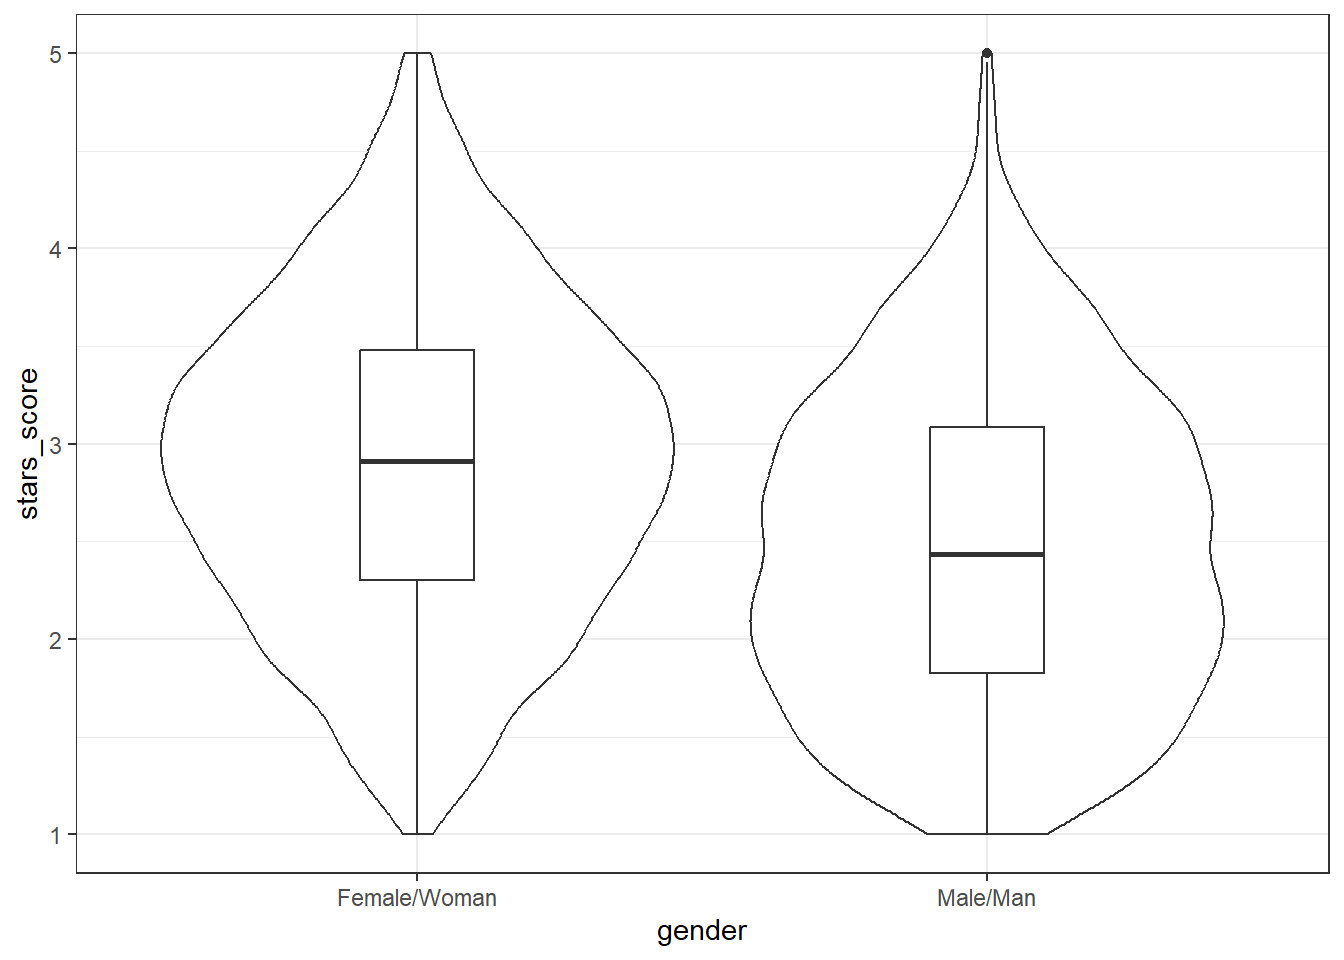
\includegraphics[width=1\linewidth]{02-webinar_files/figure-latex/unnamed-chunk-11-1} \end{center}

\subsection{Two Continuous Variables}\label{two-continuous-variables}

When working with \textbf{two continuous variables}, the primary objective of visualisation is to explore their \textbf{relationship or association}. The most commonly used plot for this purpose is the \textbf{scatterplot}, which places one variable on the x-axis and the other on the y-axis, with each point representing a single observation.

Scatterplots are particularly valuable for assessing the \textbf{form, direction, and strength of relationships} between two variables. Patterns in the data---such as linear or non-linear trends, clusters, or outliers---can often be detected visually before any formal statistical modelling is applied. A positively sloped pattern, for example, may suggest a direct relationship between variables, while a negatively sloped one may indicate an inverse relationship. Curvilinear or segmented trends may suggest more complex interactions that warrant further exploration.

One common extension of the basic scatterplot involves the addition of a \textbf{fitted line}, such as a linear regression line, to summarise the general trend in the data. This can assist viewers in interpreting the relationship more easily, especially when the raw data points are numerous or variable. A confidence interval is often included around the line to provide a visual sense of uncertainty about the estimated trend.

In many cases, it is also informative to \textbf{introduce a third variable}, typically a categorical variable, into the visualisation using \textbf{colour or shape}. This enables the examination of whether the relationship between the two continuous variables differs across groups. For example, one might investigate whether the association between anxiety and uncertainty varies by gender or age group. These grouped scatterplots are especially powerful when investigating interactions or potential moderating effects.

However, introducing grouping variables requires caution. Overplotting---where too many points obscure one another---can make the visualisation difficult to interpret. In such cases, techniques such as transparency (alpha blending), point jittering, or the use of smaller point sizes can improve readability. Alternatively, \textbf{faceting} may be used to split the plot into panels by group, allowing for clear, group-specific visualisations while preserving the structure of the original scatterplot.

\subsubsection{Scatterplots}\label{scatterplots}

\begin{Shaded}
\begin{Highlighting}[]
\CommentTok{\# simple scatterplot}
\FunctionTok{ggplot}\NormalTok{(dat\_final, }\FunctionTok{aes}\NormalTok{(}\AttributeTok{x =}\NormalTok{ stars\_score, }\AttributeTok{y =}\NormalTok{ ius\_score)) }\SpecialCharTok{+}
  \FunctionTok{geom\_point}\NormalTok{()}
\end{Highlighting}
\end{Shaded}

\begin{center}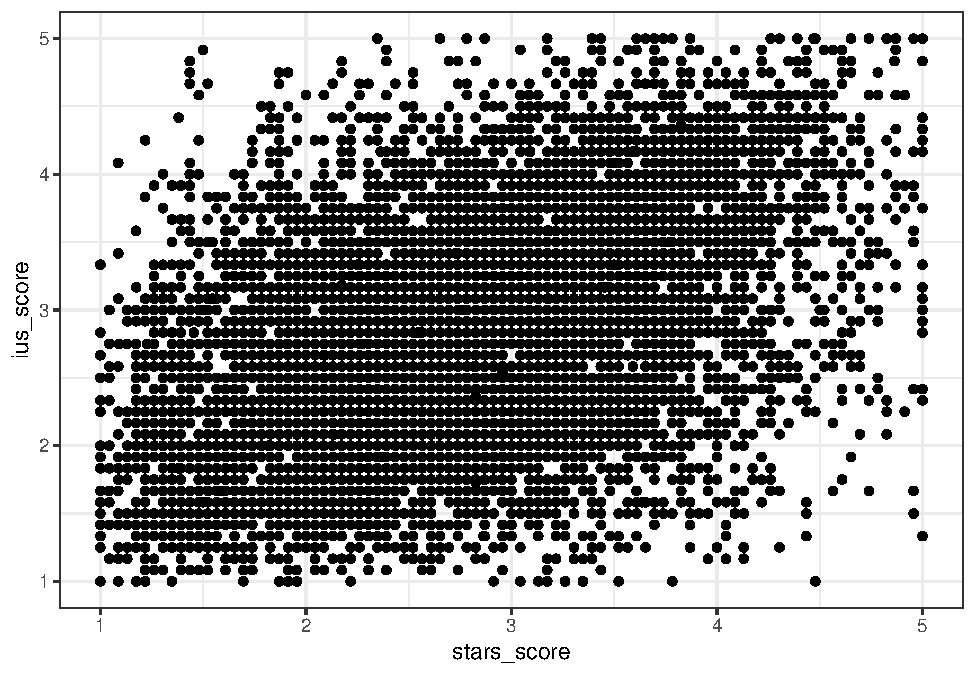
\includegraphics[width=1\linewidth]{02-webinar_files/figure-latex/unnamed-chunk-12-1} \end{center}

\begin{Shaded}
\begin{Highlighting}[]
\CommentTok{\# add line of best fit}
\FunctionTok{ggplot}\NormalTok{(dat\_final, }\FunctionTok{aes}\NormalTok{(}\AttributeTok{x =}\NormalTok{ stars\_score, }\AttributeTok{y =}\NormalTok{ ius\_score)) }\SpecialCharTok{+}
  \FunctionTok{geom\_point}\NormalTok{() }\SpecialCharTok{+}
  \FunctionTok{geom\_smooth}\NormalTok{(}\AttributeTok{method =} \StringTok{"lm"}\NormalTok{)}
\end{Highlighting}
\end{Shaded}

\begin{verbatim}
## `geom_smooth()` using formula = 'y ~ x'
\end{verbatim}

\begin{center}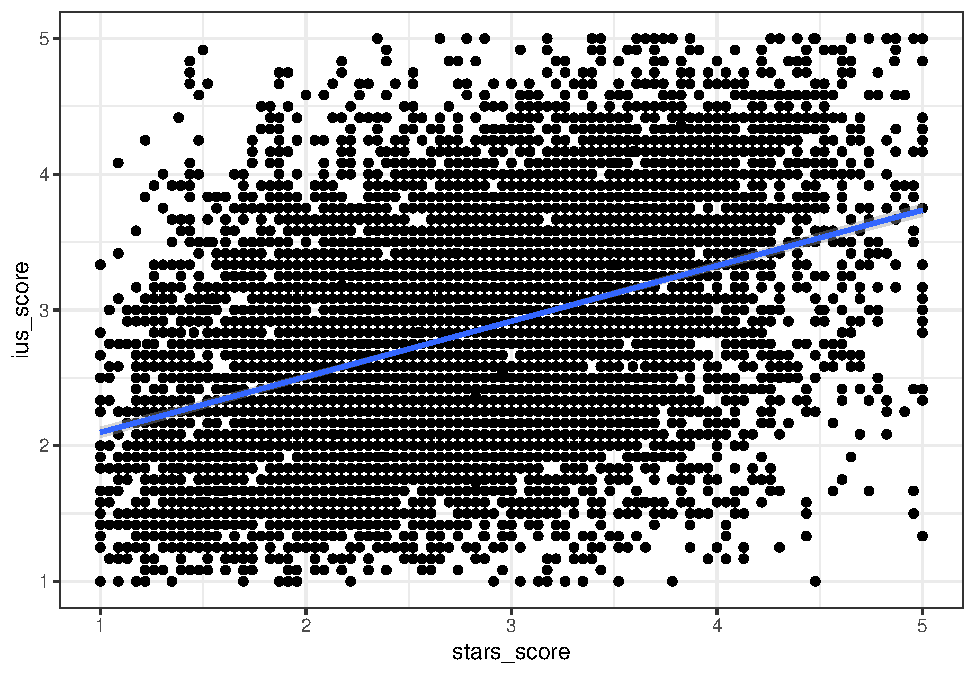
\includegraphics[width=1\linewidth]{02-webinar_files/figure-latex/unnamed-chunk-12-2} \end{center}

\begin{Shaded}
\begin{Highlighting}[]
\CommentTok{\# add in a grouping variable to all geoms}
\FunctionTok{ggplot}\NormalTok{(dat\_final, }\FunctionTok{aes}\NormalTok{(}\AttributeTok{x =}\NormalTok{ stars\_score, }\AttributeTok{y =}\NormalTok{ ius\_score, }\AttributeTok{colour =}\NormalTok{ gender)) }\SpecialCharTok{+}
  \FunctionTok{geom\_point}\NormalTok{() }\SpecialCharTok{+}
  \FunctionTok{geom\_smooth}\NormalTok{(}\AttributeTok{method =} \StringTok{"lm"}\NormalTok{)}
\end{Highlighting}
\end{Shaded}

\begin{verbatim}
## `geom_smooth()` using formula = 'y ~ x'
\end{verbatim}

\begin{center}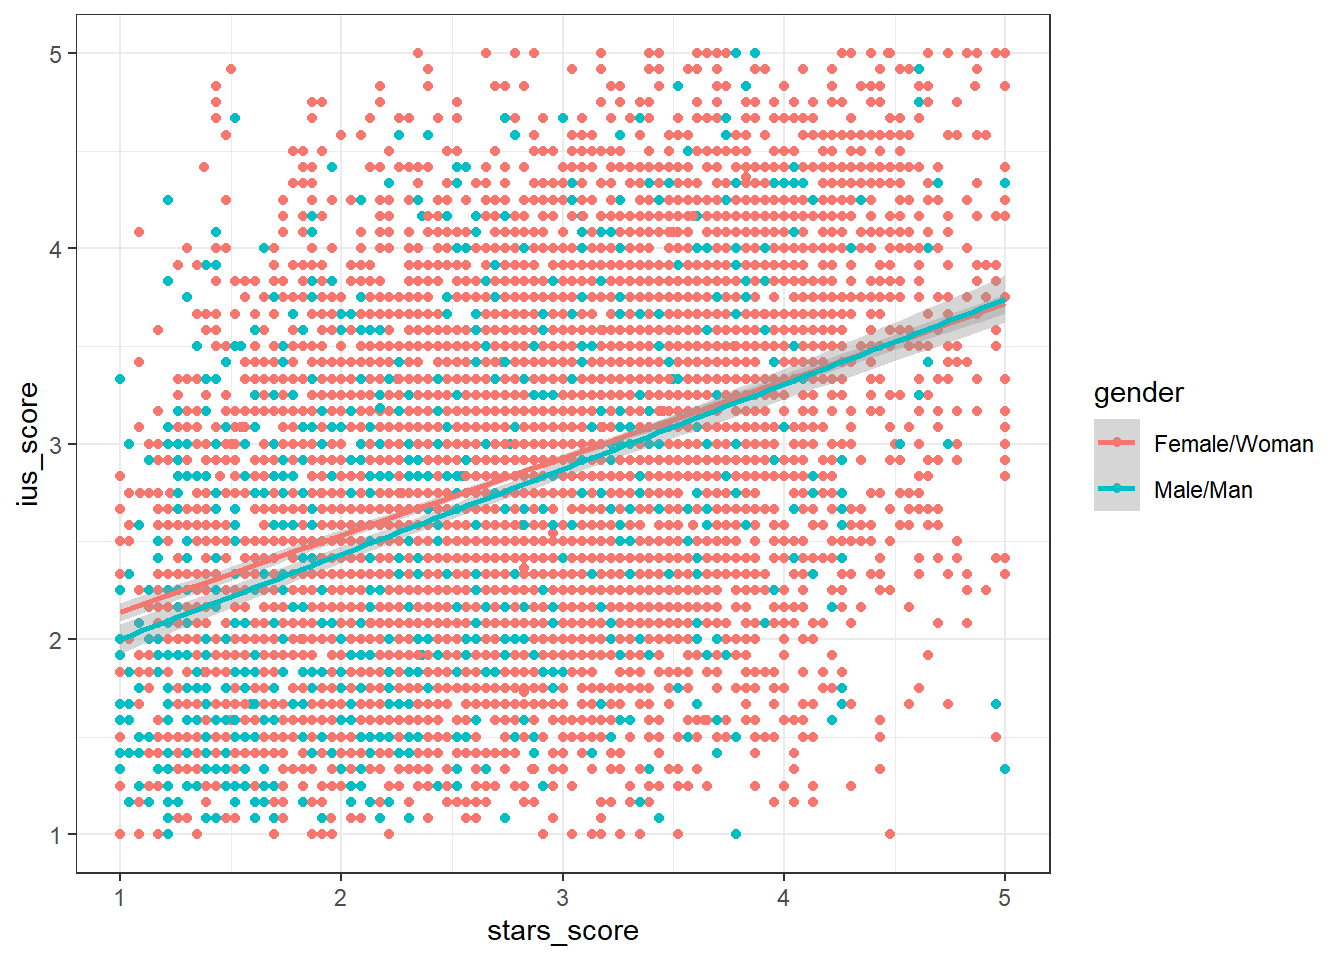
\includegraphics[width=1\linewidth]{02-webinar_files/figure-latex/unnamed-chunk-12-3} \end{center}

\begin{Shaded}
\begin{Highlighting}[]
\CommentTok{\# add in a grouping variable to one geom}
\FunctionTok{ggplot}\NormalTok{(dat\_final, }\FunctionTok{aes}\NormalTok{(}\AttributeTok{x =}\NormalTok{ stars\_score, }\AttributeTok{y =}\NormalTok{ ius\_score)) }\SpecialCharTok{+}
  \FunctionTok{geom\_point}\NormalTok{() }\SpecialCharTok{+}
  \FunctionTok{geom\_smooth}\NormalTok{(}\FunctionTok{aes}\NormalTok{(}\AttributeTok{colour =}\NormalTok{ gender), }\AttributeTok{method =} \StringTok{"lm"}\NormalTok{)}
\end{Highlighting}
\end{Shaded}

\begin{verbatim}
## `geom_smooth()` using formula = 'y ~ x'
\end{verbatim}

\begin{center}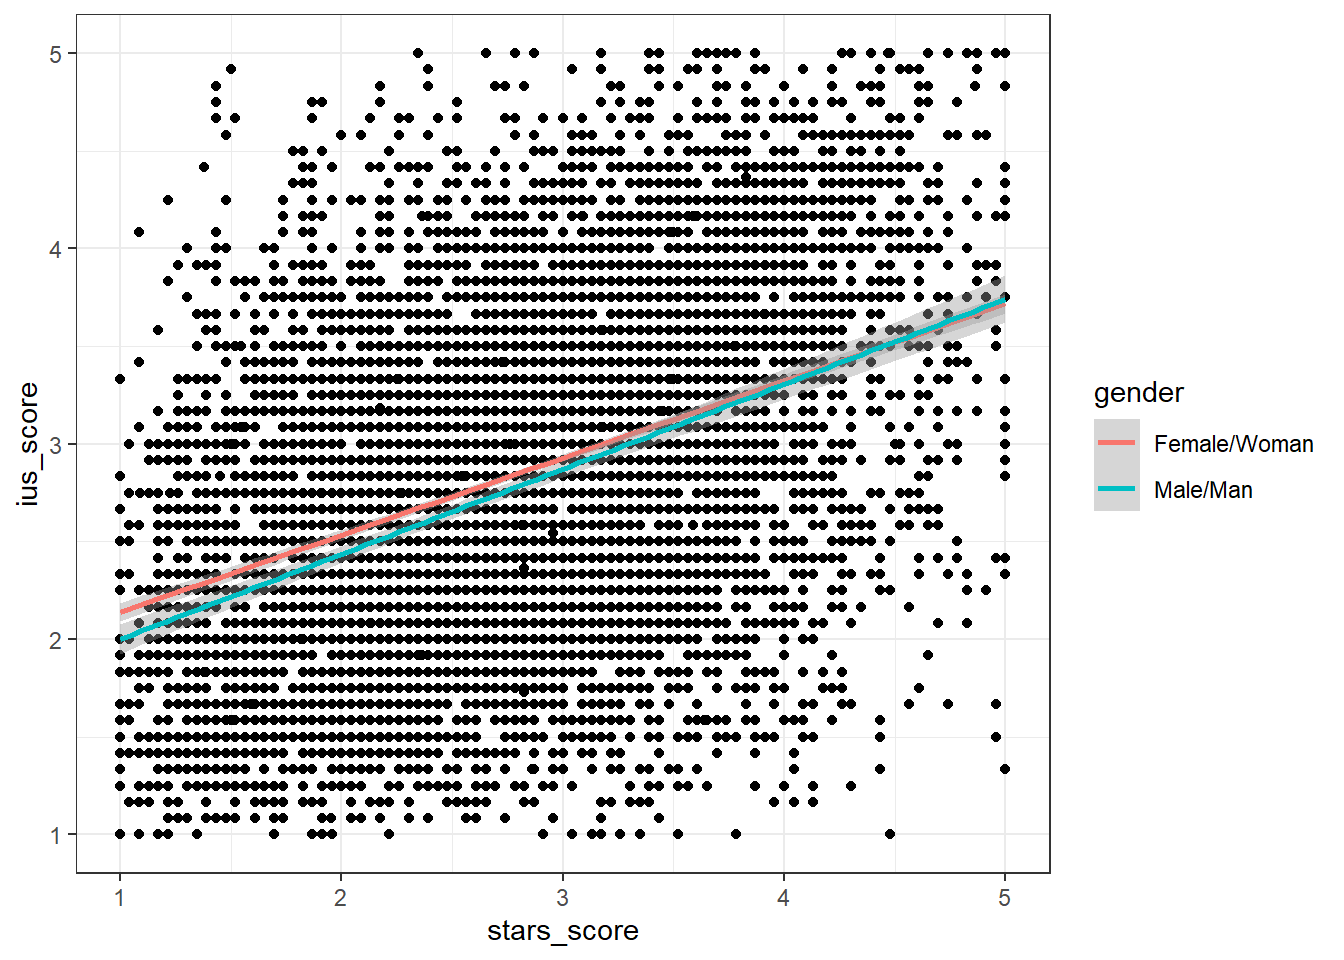
\includegraphics[width=1\linewidth]{02-webinar_files/figure-latex/unnamed-chunk-12-4} \end{center}

\section{Making it look nice}\label{making-it-look-nice}

\subsection{Titles and labels}\label{titles-and-labels}

Clear and descriptive titles and axis labels are essential for effective data visualisation. They help the viewer interpret the plot accurately and quickly. A well-chosen title conveys the main message of the plot, while subtitles can provide additional context or interpretative guidance, such as indicating the nature or direction of a relationship.

Axis labels should clearly identify the variables being plotted and include appropriate units if applicable. Avoid abbreviations or overly technical terms unless they are familiar to your audience. Good labelling ensures that your visualisations can be understood without requiring explanation from the presenter or accompanying text.

The \texttt{labs()} function in \texttt{ggplot2} allows you to specify the title, subtitle, axis labels, caption, and legend titles, all in a single place. This function should be used as part of a consistent practice of annotating all plots clearly and professionally.

\begin{Shaded}
\begin{Highlighting}[]
\FunctionTok{ggplot}\NormalTok{(dat\_final, }\FunctionTok{aes}\NormalTok{(}\AttributeTok{x =}\NormalTok{ stars\_score, }\AttributeTok{y =}\NormalTok{ ius\_score)) }\SpecialCharTok{+}
  \FunctionTok{geom\_point}\NormalTok{() }\SpecialCharTok{+}
  \FunctionTok{geom\_smooth}\NormalTok{(}\AttributeTok{method =} \StringTok{"lm"}\NormalTok{) }\SpecialCharTok{+}
  \FunctionTok{labs}\NormalTok{(}\AttributeTok{title =} \StringTok{"Relationship between IUS and STARS"}\NormalTok{,}
       \AttributeTok{subtitle =} \StringTok{"Positive correlation"}\NormalTok{,}
       \AttributeTok{x =} \StringTok{"Statistics Anxiety Score"}\NormalTok{,}
       \AttributeTok{y =} \StringTok{"Intolerance of Uncertainity Score"}\NormalTok{)}
\end{Highlighting}
\end{Shaded}

\begin{verbatim}
## `geom_smooth()` using formula = 'y ~ x'
\end{verbatim}

\begin{center}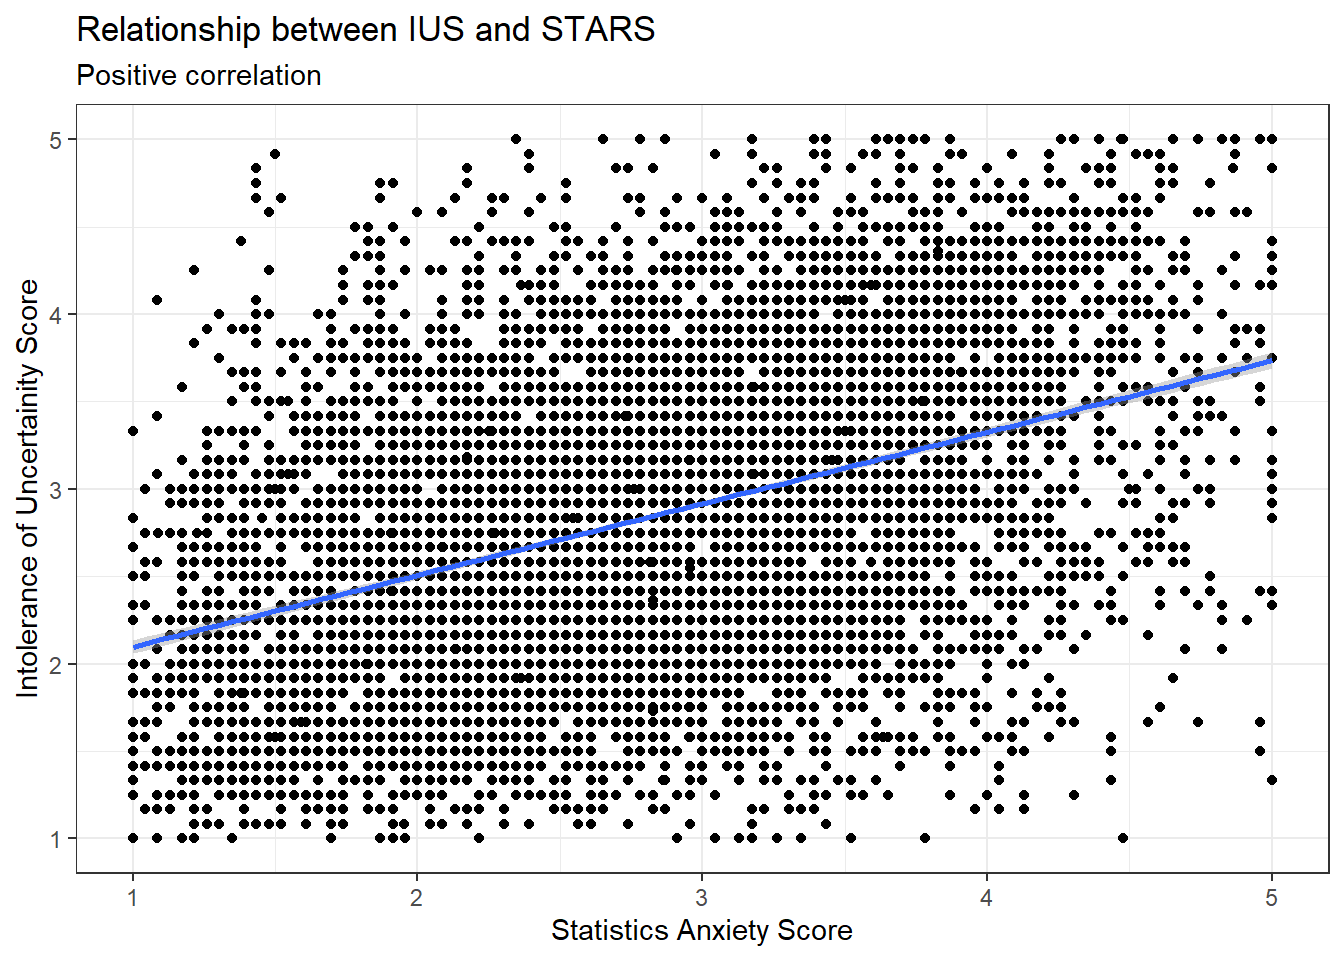
\includegraphics[width=1\linewidth]{02-webinar_files/figure-latex/unnamed-chunk-13-1} \end{center}

\subsection{Adding a theme}\label{adding-a-theme}

Themes in \texttt{ggplot2} control the \textbf{non-data elements} of a plot---such as background colour, gridlines, font size, margins, and axis line styles. By default, \texttt{ggplot2} applies the \texttt{theme\_grey()} theme, which uses a grey background and white gridlines. While this is functional, other themes can often improve clarity or align better with publication standards.

The choice of theme can have a substantial impact on the visual appeal and readability of a plot. For example, \texttt{theme\_minimal()} offers a clean, white background with minimal distraction, making it ideal for presentations and teaching. \texttt{theme\_classic()} provides a more traditional, academic appearance, resembling hand-drawn plots or older textbook figures. Alternatively, the \texttt{theme\_apa()} from the \texttt{jtools} package adheres to the American Psychological Association's publication style, which is particularly helpful in psychology and related disciplines.

Consistent use of themes across all plots in a project or presentation contributes to a professional and cohesive visual identity. It also helps focus the viewer's attention on the data, rather than on stylistic inconsistencies or extraneous visual elements.

\begin{Shaded}
\begin{Highlighting}[]
\CommentTok{\# theme\_minimal from ggplot}
\FunctionTok{ggplot}\NormalTok{(dat\_final, }\FunctionTok{aes}\NormalTok{(}\AttributeTok{x =}\NormalTok{ stars\_score, }\AttributeTok{y =}\NormalTok{ ius\_score)) }\SpecialCharTok{+}
  \FunctionTok{geom\_point}\NormalTok{() }\SpecialCharTok{+}
  \FunctionTok{geom\_smooth}\NormalTok{(}\AttributeTok{method =} \StringTok{"lm"}\NormalTok{) }\SpecialCharTok{+}
  \FunctionTok{labs}\NormalTok{(}\AttributeTok{title =} \StringTok{"Relationship between IUS and STARS"}\NormalTok{,}
       \AttributeTok{subtitle =} \StringTok{"Positive correlation"}\NormalTok{,}
       \AttributeTok{x =} \StringTok{"Statistics Anxiety Score"}\NormalTok{,}
       \AttributeTok{y =} \StringTok{"Intolerance of Uncertainity Score"}\NormalTok{) }\SpecialCharTok{+}
  \FunctionTok{theme\_minimal}\NormalTok{()}
\end{Highlighting}
\end{Shaded}

\begin{verbatim}
## `geom_smooth()` using formula = 'y ~ x'
\end{verbatim}

\begin{center}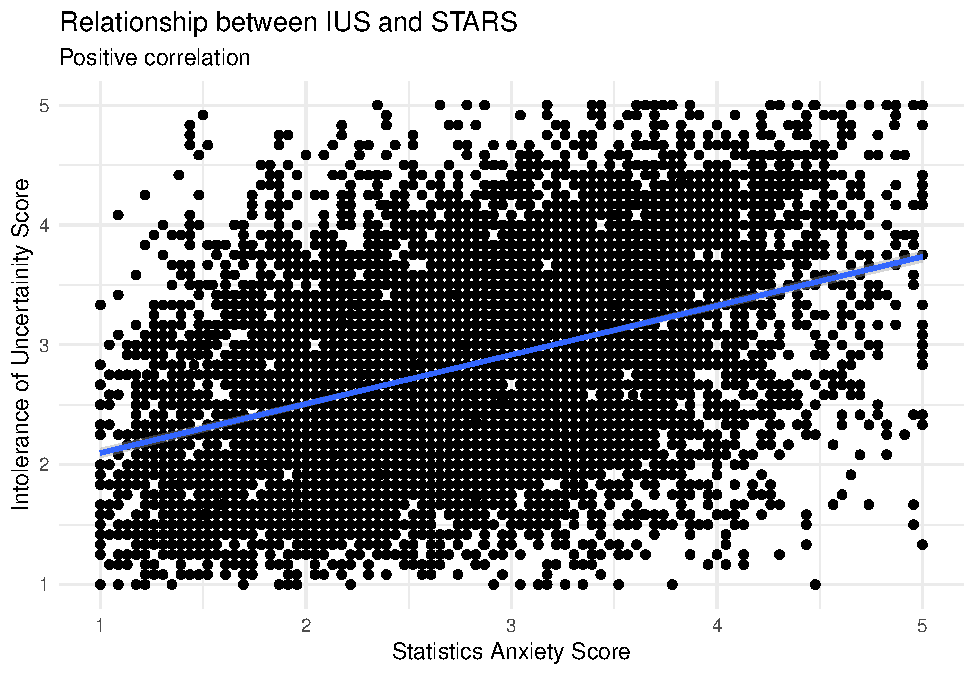
\includegraphics[width=1\linewidth]{02-webinar_files/figure-latex/unnamed-chunk-14-1} \end{center}

\begin{Shaded}
\begin{Highlighting}[]
\CommentTok{\# theme\_classic from ggplot}
\FunctionTok{ggplot}\NormalTok{(dat\_final, }\FunctionTok{aes}\NormalTok{(}\AttributeTok{x =}\NormalTok{ stars\_score, }\AttributeTok{y =}\NormalTok{ ius\_score)) }\SpecialCharTok{+}
  \FunctionTok{geom\_point}\NormalTok{() }\SpecialCharTok{+}
  \FunctionTok{geom\_smooth}\NormalTok{(}\AttributeTok{method =} \StringTok{"lm"}\NormalTok{) }\SpecialCharTok{+}
  \FunctionTok{labs}\NormalTok{(}\AttributeTok{title =} \StringTok{"Relationship between IUS and STARS"}\NormalTok{,}
       \AttributeTok{subtitle =} \StringTok{"Positive correlation"}\NormalTok{,}
       \AttributeTok{x =} \StringTok{"Statistics Anxiety Score"}\NormalTok{,}
       \AttributeTok{y =} \StringTok{"Intolerance of Uncertainity Score"}\NormalTok{) }\SpecialCharTok{+}
  \FunctionTok{theme\_classic}\NormalTok{()}
\end{Highlighting}
\end{Shaded}

\begin{verbatim}
## `geom_smooth()` using formula = 'y ~ x'
\end{verbatim}

\begin{center}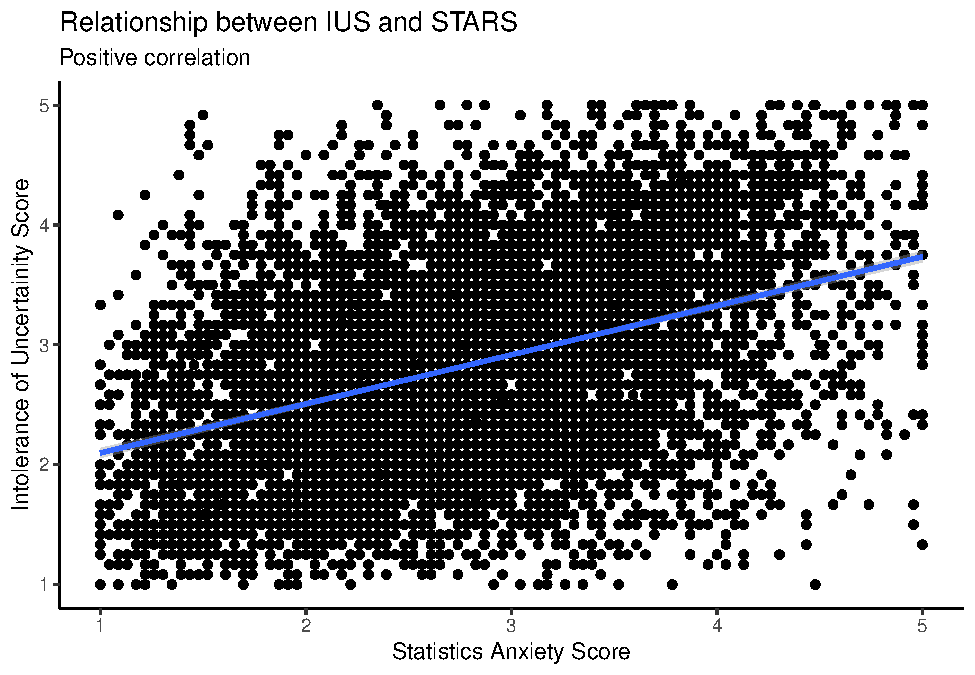
\includegraphics[width=1\linewidth]{02-webinar_files/figure-latex/unnamed-chunk-14-2} \end{center}

\begin{Shaded}
\begin{Highlighting}[]
\CommentTok{\# apa theme from jtools}
\FunctionTok{ggplot}\NormalTok{(dat\_final, }\FunctionTok{aes}\NormalTok{(}\AttributeTok{x =}\NormalTok{ stars\_score, }\AttributeTok{y =}\NormalTok{ ius\_score)) }\SpecialCharTok{+}
  \FunctionTok{geom\_point}\NormalTok{() }\SpecialCharTok{+}
  \FunctionTok{geom\_smooth}\NormalTok{(}\AttributeTok{method =} \StringTok{"lm"}\NormalTok{) }\SpecialCharTok{+}
  \FunctionTok{labs}\NormalTok{(}\AttributeTok{title =} \StringTok{"Relationship between IUS and STARS"}\NormalTok{,}
       \AttributeTok{subtitle =} \StringTok{"Positive correlation"}\NormalTok{,}
       \AttributeTok{x =} \StringTok{"Statistics Anxiety Score"}\NormalTok{,}
       \AttributeTok{y =} \StringTok{"Intolerance of Uncertainity Score"}\NormalTok{) }\SpecialCharTok{+}
  \FunctionTok{theme\_apa}\NormalTok{()}
\end{Highlighting}
\end{Shaded}

\begin{verbatim}
## `geom_smooth()` using formula = 'y ~ x'
\end{verbatim}

\begin{center}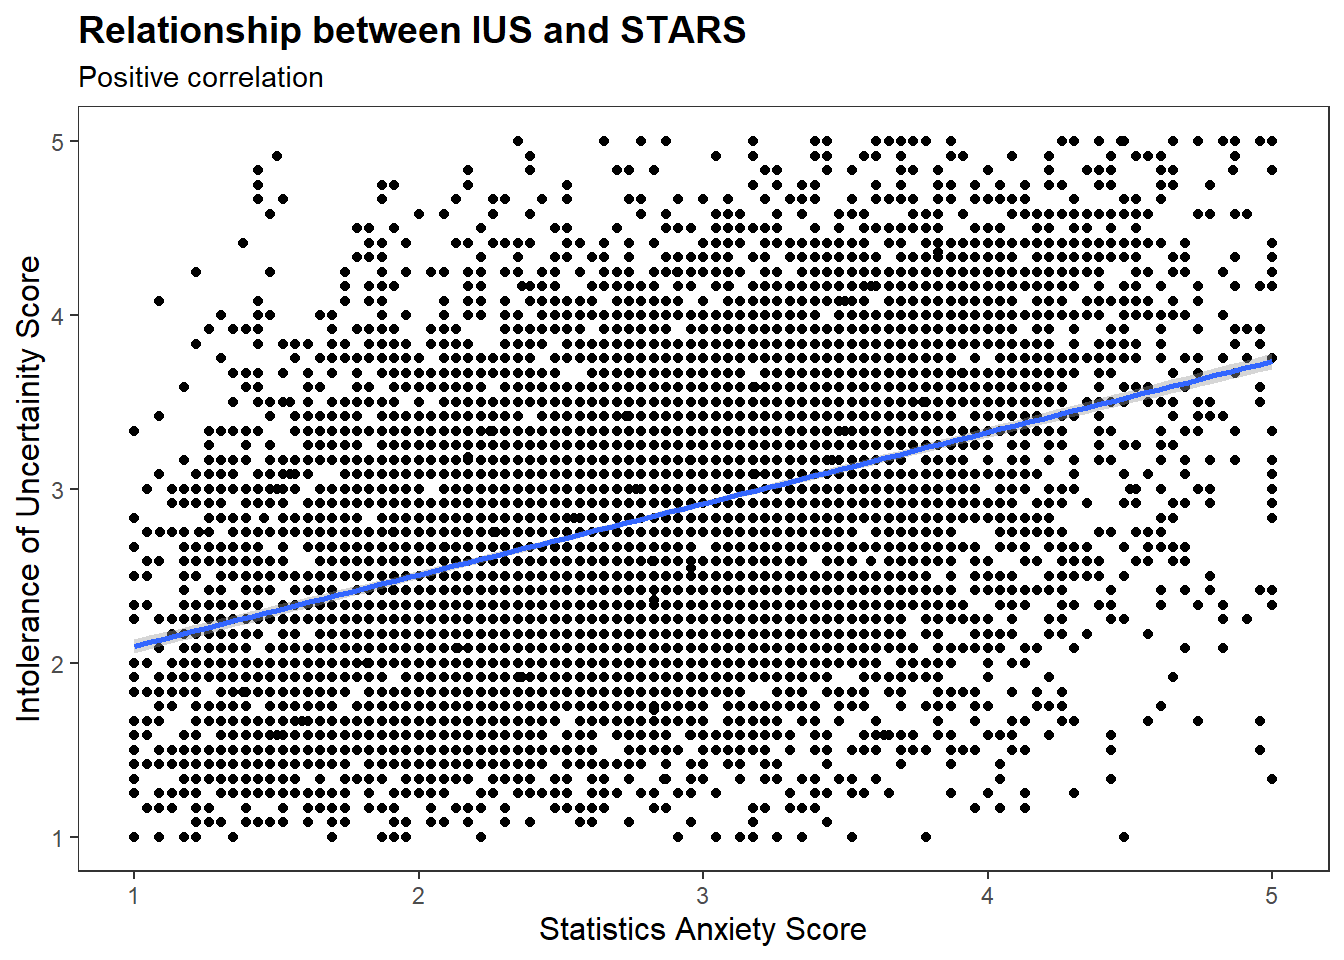
\includegraphics[width=1\linewidth]{02-webinar_files/figure-latex/unnamed-chunk-14-3} \end{center}

\subsection{Adding colour}\label{adding-colour}

Colour is a powerful tool in data visualisation, capable of highlighting group differences, drawing attention to key patterns, and improving interpretability. However, it must be used judiciously. When introducing colour, it is important to ensure that it adds meaningful information and does not create unnecessary visual clutter or redundancy.

In many cases, the default behaviour of \texttt{ggplot2} will include a colour legend when a grouping variable is mapped to an aesthetic such as \texttt{fill} or \texttt{colour}. If this grouping is already evident from the axis (e.g., when grouping is shown along the x-axis), the legend may be redundant. Removing it can make the plot cleaner and more space-efficient, particularly in slide-based or publication formats.

Colour choice should also take accessibility into account. For example, using a \textbf{colour-blind friendly palette}, such as \texttt{"Dark2"} from the \texttt{RColorBrewer} package, ensures that plots are interpretable by a wider audience, including those with common forms of colour vision deficiency. This is a critical consideration in inclusive teaching and communication.

Finally, when the default palettes do not meet the presentational needs or aesthetic preferences of the analyst, colours can be specified manually. This provides full control over the visual appearance and is particularly useful when aligning plots with institutional branding or publication requirements.

\begin{Shaded}
\begin{Highlighting}[]
\CommentTok{\# add colour, remove legend}
\FunctionTok{ggplot}\NormalTok{(dat\_final, }\FunctionTok{aes}\NormalTok{(}\AttributeTok{x =}\NormalTok{ gender, }\AttributeTok{y =}\NormalTok{ stars\_score, }\AttributeTok{fill =}\NormalTok{ gender)) }\SpecialCharTok{+}
  \FunctionTok{geom\_boxplot}\NormalTok{() }\SpecialCharTok{+}
  \FunctionTok{guides}\NormalTok{(}\AttributeTok{fill =} \StringTok{"none"}\NormalTok{)}
\end{Highlighting}
\end{Shaded}

\begin{center}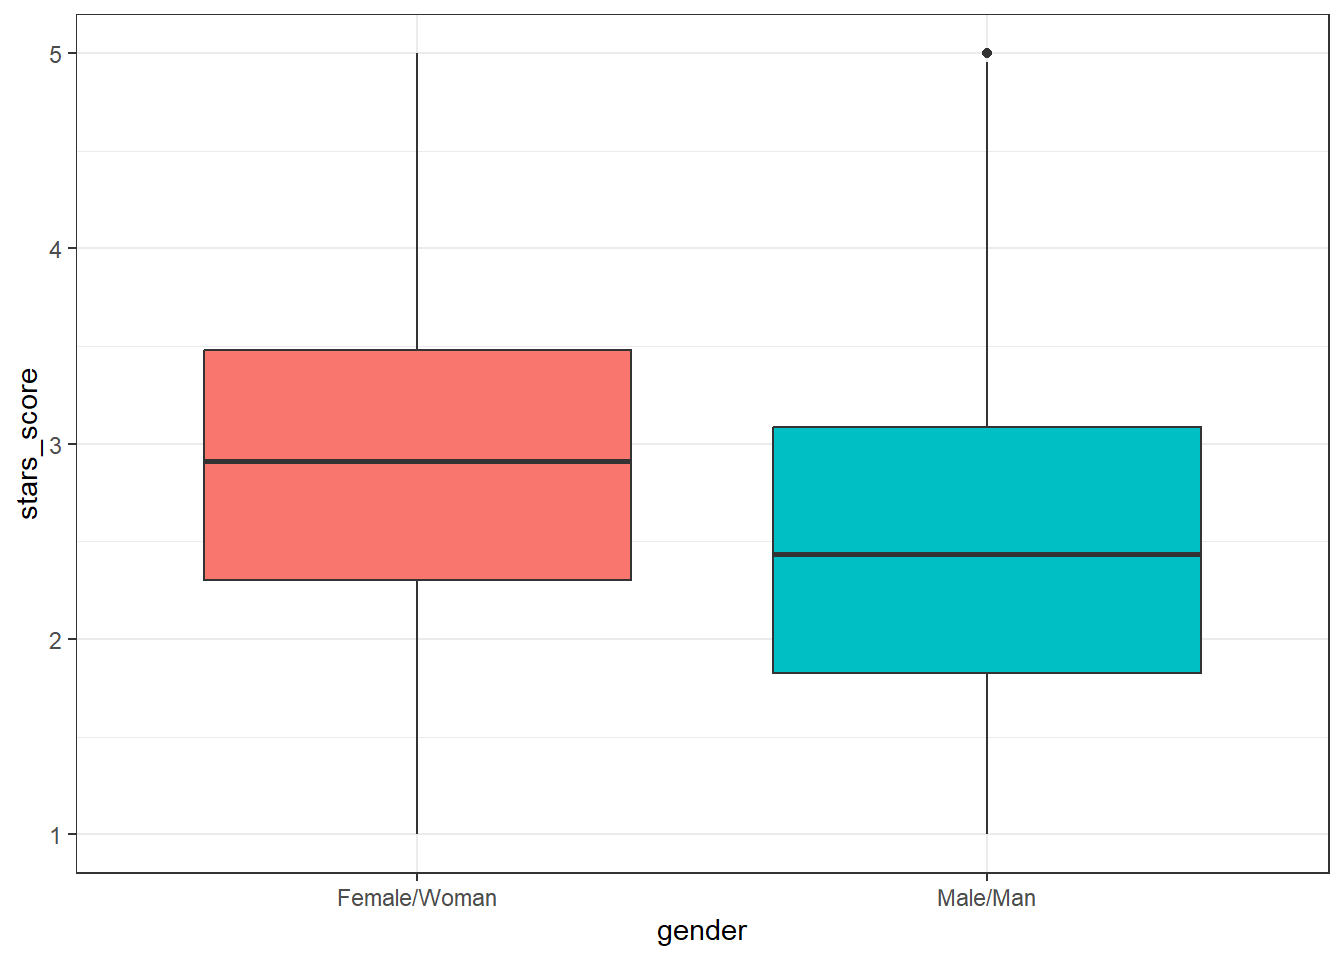
\includegraphics[width=1\linewidth]{02-webinar_files/figure-latex/unnamed-chunk-15-1} \end{center}

\begin{Shaded}
\begin{Highlighting}[]
\CommentTok{\# use a colour blind friendly palette}

\FunctionTok{ggplot}\NormalTok{(dat\_final, }\FunctionTok{aes}\NormalTok{(}\AttributeTok{x =}\NormalTok{ gender, }\AttributeTok{y =}\NormalTok{ stars\_score, }\AttributeTok{fill =}\NormalTok{ gender)) }\SpecialCharTok{+}
  \FunctionTok{geom\_boxplot}\NormalTok{() }\SpecialCharTok{+}
  \FunctionTok{guides}\NormalTok{(}\AttributeTok{fill =} \StringTok{"none"}\NormalTok{) }\SpecialCharTok{+}
  \FunctionTok{scale\_fill\_brewer}\NormalTok{(}\AttributeTok{palette =} \StringTok{"Dark2"}\NormalTok{)}
\end{Highlighting}
\end{Shaded}

\begin{center}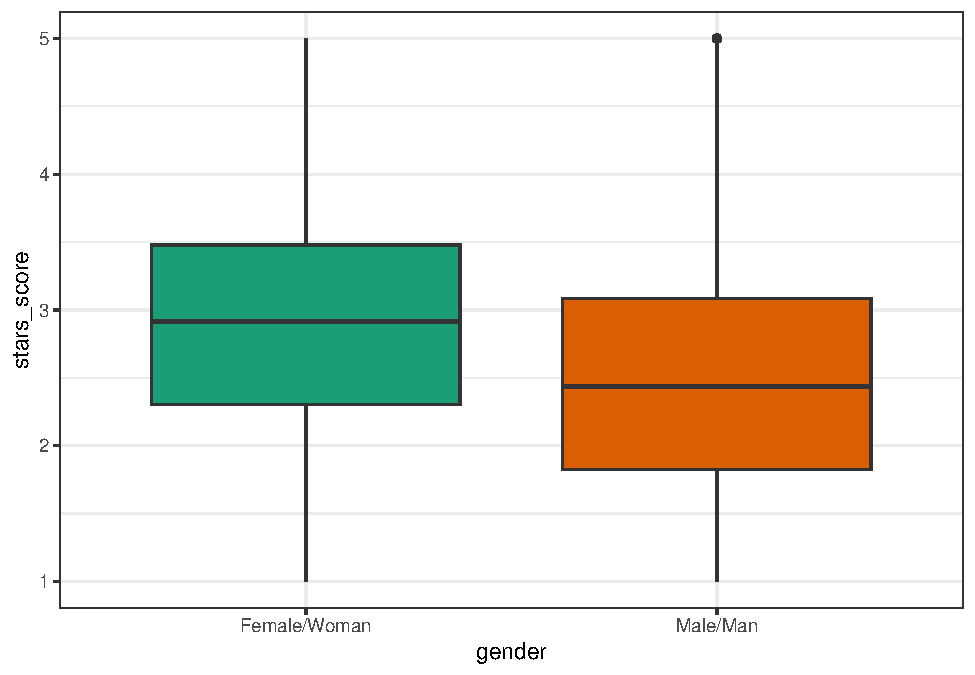
\includegraphics[width=1\linewidth]{02-webinar_files/figure-latex/unnamed-chunk-15-2} \end{center}

\begin{Shaded}
\begin{Highlighting}[]
\CommentTok{\# specify colour manually}

\FunctionTok{ggplot}\NormalTok{(dat\_final, }\FunctionTok{aes}\NormalTok{(}\AttributeTok{x =}\NormalTok{ gender, }\AttributeTok{y =}\NormalTok{ stars\_score, }\AttributeTok{fill =}\NormalTok{ gender)) }\SpecialCharTok{+}
  \FunctionTok{geom\_boxplot}\NormalTok{() }\SpecialCharTok{+}
  \FunctionTok{guides}\NormalTok{(}\AttributeTok{fill =} \StringTok{"none"}\NormalTok{) }\SpecialCharTok{+}
  \FunctionTok{scale\_fill\_manual}\NormalTok{(}\AttributeTok{values =} \FunctionTok{c}\NormalTok{(}\StringTok{"darkgrey"}\NormalTok{, }\StringTok{"lightblue"}\NormalTok{))}
\end{Highlighting}
\end{Shaded}

\begin{center}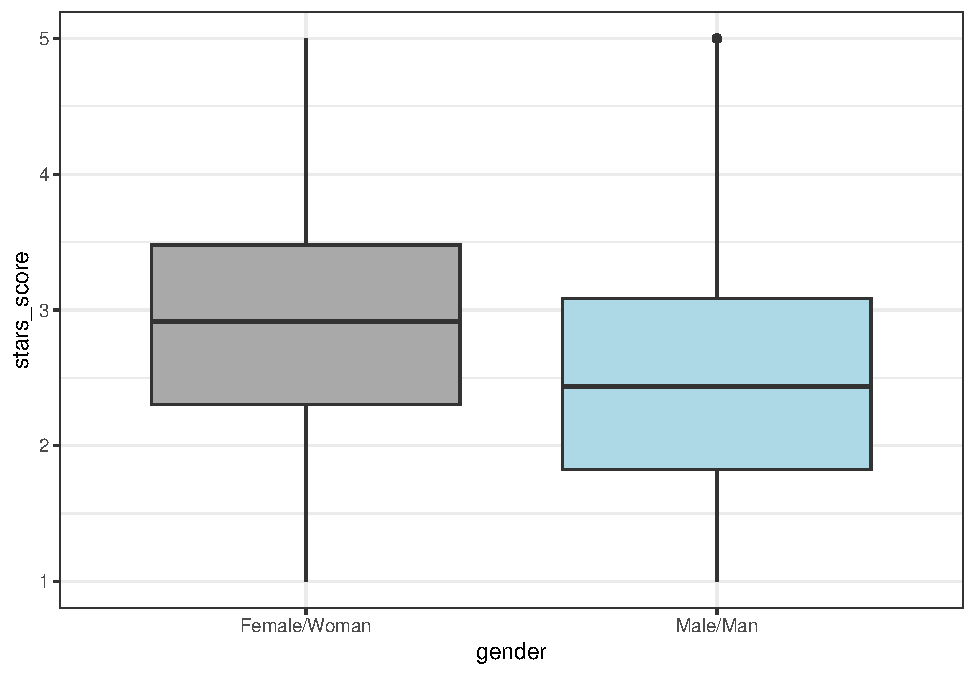
\includegraphics[width=1\linewidth]{02-webinar_files/figure-latex/unnamed-chunk-15-3} \end{center}

\subsection{Editing the scale}\label{editing-the-scale}

Scale functions in \texttt{ggplot2} control how data values are mapped to visual properties such as position, colour, or size. When used thoughtfully, editing the scale can significantly improve the interpretability and precision of a plot.

One common modification is adjusting the \textbf{breaks} on an axis. This allows the analyst to specify exactly where tick marks should appear, which can aid interpretation and consistency across plots---especially when comparing multiple figures side by side. For example, specifying regular intervals (e.g., every 0.5 units) on a continuous scale can make trends more apparent and reduce cognitive load for the viewer.

In addition to breaks, \textbf{axis labels} may need to be edited to improve clarity or accessibility. For categorical axes, this often involves renaming factor levels to use plain language or more inclusive terminology. However, it is important to ensure that the order of labels matches the underlying factor levels in the data to avoid unintended mismatches or misinterpretation.

Another common modification is setting \textbf{limits} on a scale, which controls the minimum and maximum values displayed on an axis. This can be useful for focusing the viewer's attention on a relevant range or ensuring that multiple plots share the same axis limits for valid comparison. That said, limits should be chosen carefully to avoid omitting important data or misleading the viewer by exaggerating or minimising differences.

\begin{Shaded}
\begin{Highlighting}[]
\CommentTok{\# change the breaks}
\FunctionTok{ggplot}\NormalTok{(}\AttributeTok{data =}\NormalTok{ dat\_final, }\FunctionTok{aes}\NormalTok{(stars\_score)) }\SpecialCharTok{+}
  \FunctionTok{geom\_histogram}\NormalTok{(}\AttributeTok{binwidth =}\NormalTok{ .}\DecValTok{25}\NormalTok{, }
                 \AttributeTok{boundary =} \DecValTok{0}\NormalTok{, }
                 \AttributeTok{colour =} \StringTok{"black"}\NormalTok{,}
                 \AttributeTok{fill =} \StringTok{"lightblue"}\NormalTok{) }\SpecialCharTok{+}
  \FunctionTok{scale\_x\_continuous}\NormalTok{(}\AttributeTok{breaks =} \FunctionTok{seq}\NormalTok{(}\AttributeTok{from =} \DecValTok{1}\NormalTok{, }\AttributeTok{to =} \DecValTok{5}\NormalTok{, }\AttributeTok{by =} \FloatTok{0.5}\NormalTok{))}
\end{Highlighting}
\end{Shaded}

\begin{center}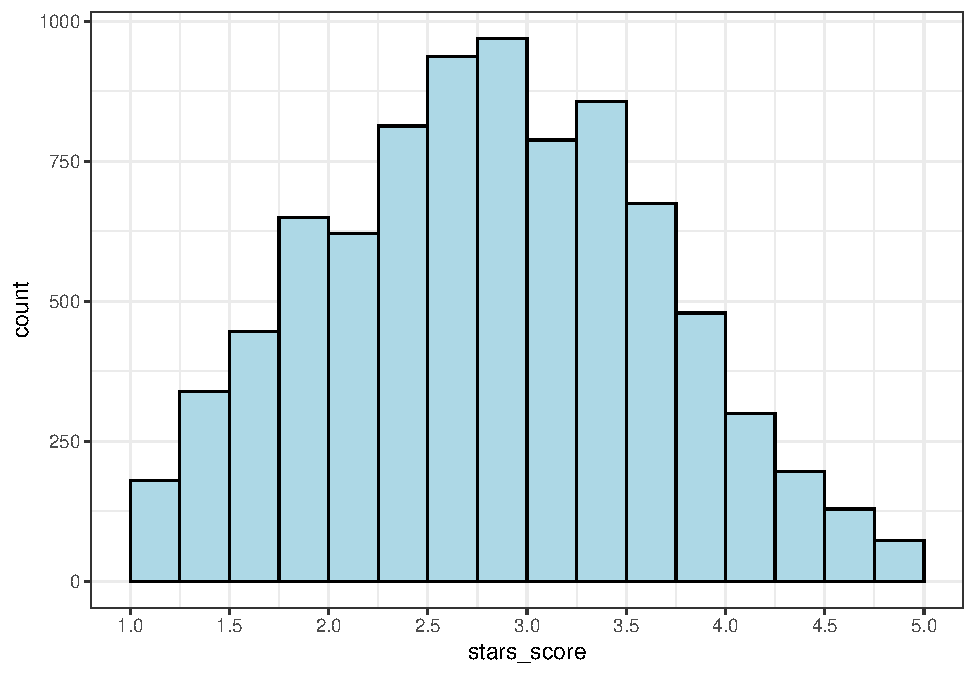
\includegraphics[width=1\linewidth]{02-webinar_files/figure-latex/unnamed-chunk-16-1} \end{center}

\begin{Shaded}
\begin{Highlighting}[]
\CommentTok{\# changing the labels {-} be careful of order!}
\FunctionTok{ggplot}\NormalTok{(dat\_final, }\FunctionTok{aes}\NormalTok{(}\AttributeTok{x =}\NormalTok{ gender, }\AttributeTok{y =}\NormalTok{ stars\_score, }\AttributeTok{fill =}\NormalTok{ gender)) }\SpecialCharTok{+}
  \FunctionTok{geom\_boxplot}\NormalTok{() }\SpecialCharTok{+}
  \FunctionTok{guides}\NormalTok{(}\AttributeTok{fill =} \StringTok{"none"}\NormalTok{) }\SpecialCharTok{+}
  \FunctionTok{scale\_fill\_manual}\NormalTok{(}\AttributeTok{values =} \FunctionTok{c}\NormalTok{(}\StringTok{"darkgrey"}\NormalTok{, }\StringTok{"lightblue"}\NormalTok{)) }\SpecialCharTok{+}
  \FunctionTok{scale\_x\_discrete}\NormalTok{(}\AttributeTok{labels =} \FunctionTok{c}\NormalTok{(}\StringTok{"Woman"}\NormalTok{, }\StringTok{"Man"}\NormalTok{))}
\end{Highlighting}
\end{Shaded}

\begin{center}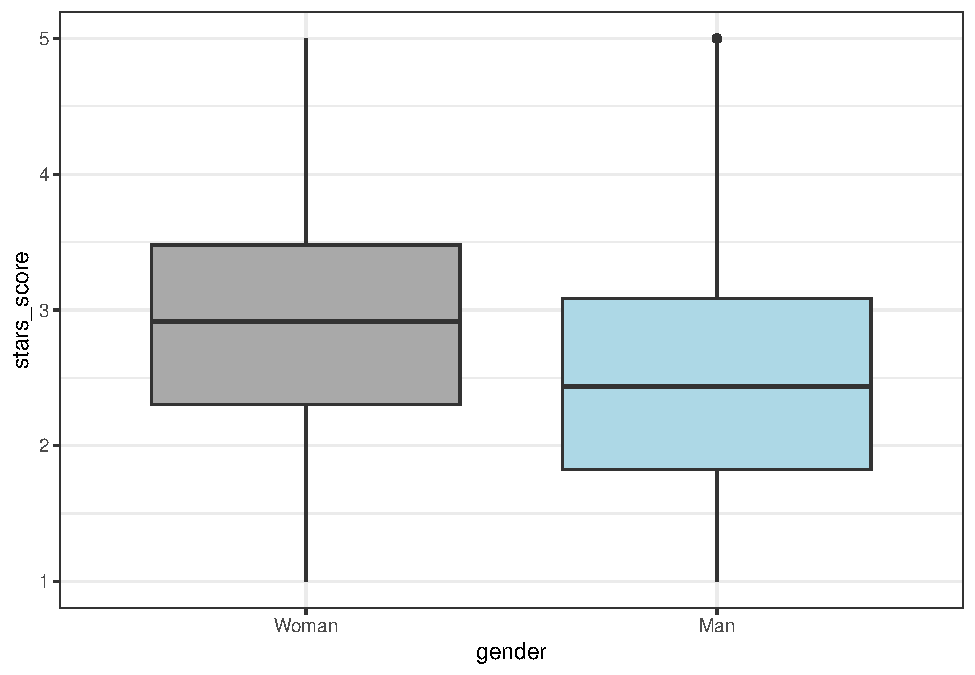
\includegraphics[width=1\linewidth]{02-webinar_files/figure-latex/unnamed-chunk-16-2} \end{center}

\begin{Shaded}
\begin{Highlighting}[]
\CommentTok{\# changing the limits}
\FunctionTok{ggplot}\NormalTok{(}\AttributeTok{data =}\NormalTok{ dat\_final, }\FunctionTok{aes}\NormalTok{(stars\_score)) }\SpecialCharTok{+}
  \FunctionTok{geom\_histogram}\NormalTok{(}\AttributeTok{binwidth =}\NormalTok{ .}\DecValTok{25}\NormalTok{, }
                 \AttributeTok{boundary =} \DecValTok{0}\NormalTok{, }
                 \AttributeTok{colour =} \StringTok{"black"}\NormalTok{,}
                 \AttributeTok{fill =} \StringTok{"lightblue"}\NormalTok{) }\SpecialCharTok{+}
  \FunctionTok{scale\_x\_continuous}\NormalTok{(}\AttributeTok{limits =} \FunctionTok{c}\NormalTok{(}\DecValTok{0}\NormalTok{,}\DecValTok{6}\NormalTok{))}
\end{Highlighting}
\end{Shaded}

\begin{center}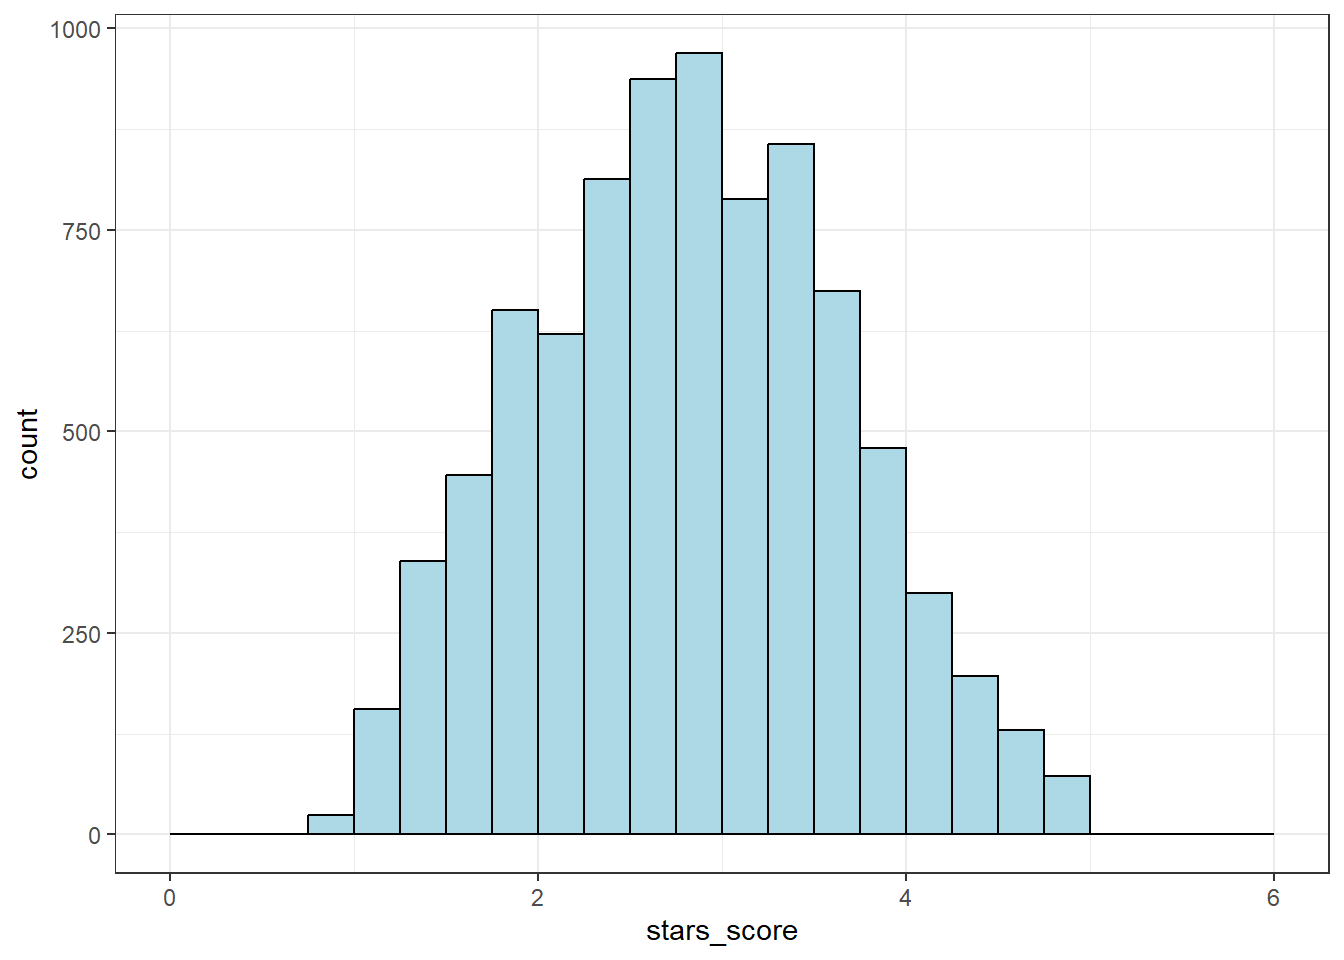
\includegraphics[width=1\linewidth]{02-webinar_files/figure-latex/unnamed-chunk-16-3} \end{center}

\section{Going a bit wild}\label{going-a-bit-wild}

\begin{Shaded}
\begin{Highlighting}[]
\CommentTok{\# changing the labels {-} be careful of order!}
\FunctionTok{ggplot}\NormalTok{(dat\_final, }\FunctionTok{aes}\NormalTok{(}\AttributeTok{x =}\NormalTok{ gender, }\AttributeTok{y =}\NormalTok{ stars\_score, }\AttributeTok{fill =}\NormalTok{ gender)) }\SpecialCharTok{+}
  \FunctionTok{geom\_jitter}\NormalTok{(}\AttributeTok{width =}\NormalTok{ .}\DecValTok{25}\NormalTok{, }\AttributeTok{height =}\NormalTok{ .}\DecValTok{2}\NormalTok{, }\AttributeTok{alpha =}\NormalTok{ .}\DecValTok{2}\NormalTok{) }\SpecialCharTok{+}
  \FunctionTok{geom\_violin}\NormalTok{(}\AttributeTok{alpha =}\NormalTok{.}\DecValTok{4}\NormalTok{) }\SpecialCharTok{+}
  \FunctionTok{geom\_boxplot}\NormalTok{() }\SpecialCharTok{+}
  \FunctionTok{stat\_summary}\NormalTok{(}\AttributeTok{fun =} \StringTok{"mean"}\NormalTok{, }\AttributeTok{geom =} \StringTok{"point"}\NormalTok{, }\AttributeTok{size =}\DecValTok{2}\NormalTok{) }\SpecialCharTok{+}
  \FunctionTok{stat\_summary}\NormalTok{(}\AttributeTok{fun.data =} \StringTok{"mean\_se"}\NormalTok{, }\AttributeTok{geom =} \StringTok{"errorbar"}\NormalTok{, }\AttributeTok{width =}\NormalTok{ .}\DecValTok{2}\NormalTok{)}\SpecialCharTok{+}
  \FunctionTok{guides}\NormalTok{(}\AttributeTok{fill =} \StringTok{"none"}\NormalTok{) }\SpecialCharTok{+}
  \FunctionTok{scale\_fill\_manual}\NormalTok{(}\AttributeTok{values =} \FunctionTok{c}\NormalTok{(}\StringTok{"darkgrey"}\NormalTok{, }\StringTok{"lightblue"}\NormalTok{)) }\SpecialCharTok{+}
  \FunctionTok{scale\_x\_discrete}\NormalTok{(}\AttributeTok{labels =} \FunctionTok{c}\NormalTok{(}\StringTok{"Woman"}\NormalTok{, }\StringTok{"Man"}\NormalTok{))}\SpecialCharTok{+}
  \FunctionTok{labs}\NormalTok{(}\AttributeTok{title =} \StringTok{"Gender differences in statistics anxiety"}\NormalTok{,}
       \AttributeTok{x =} \StringTok{"Gender"}\NormalTok{,}
       \AttributeTok{y =} \StringTok{"Statistics Anxiety Score"}\NormalTok{) }\SpecialCharTok{+}
  \FunctionTok{theme\_apa}\NormalTok{()}\SpecialCharTok{+}
  \FunctionTok{annotate}\NormalTok{(}\AttributeTok{geom =} \StringTok{"text"}\NormalTok{,}
           \AttributeTok{label =} \StringTok{"Maybe we need DEI after all"}\NormalTok{,}
           \AttributeTok{x =} \FloatTok{1.5}\NormalTok{, }\AttributeTok{y =} \FloatTok{3.5}\NormalTok{,}
           \AttributeTok{hjust =} \DecValTok{0}\NormalTok{, }\AttributeTok{vjust =} \DecValTok{1}\NormalTok{, }
           \AttributeTok{color =} \StringTok{"black"}\NormalTok{, }\AttributeTok{fontface =} \StringTok{"bold"}\NormalTok{,}
           \AttributeTok{angle =} \DecValTok{45}\NormalTok{) }
\end{Highlighting}
\end{Shaded}

\begin{center}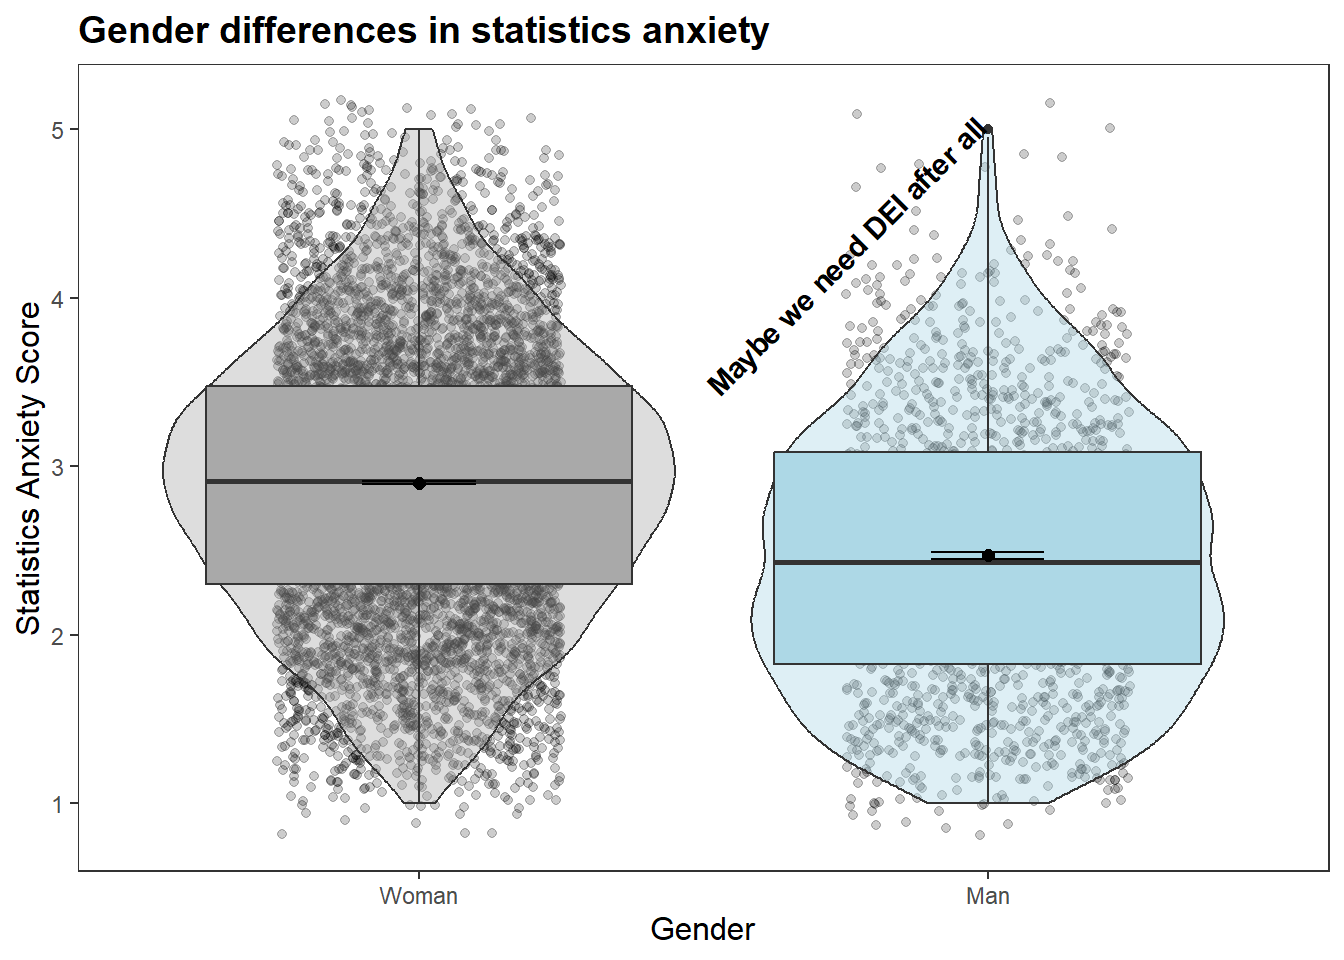
\includegraphics[width=1\linewidth]{02-webinar_files/figure-latex/unnamed-chunk-17-1} \end{center}

\begin{Shaded}
\begin{Highlighting}[]
\CommentTok{\# marginal histograms}
\NormalTok{p }\OtherTok{\textless{}{-}} \FunctionTok{ggplot}\NormalTok{(dat\_final, }\FunctionTok{aes}\NormalTok{(}\AttributeTok{x =}\NormalTok{ stars\_score, }\AttributeTok{y =}\NormalTok{ ius\_score)) }\SpecialCharTok{+}
  \FunctionTok{geom\_point}\NormalTok{() }\SpecialCharTok{+}
  \FunctionTok{geom\_smooth}\NormalTok{(}\AttributeTok{method =} \StringTok{"lm"}\NormalTok{) }\SpecialCharTok{+}
  \FunctionTok{labs}\NormalTok{(}\AttributeTok{title =} \StringTok{"Relationship between IUS and STARS"}\NormalTok{,}
       \AttributeTok{subtitle =} \StringTok{"Positive correlation"}\NormalTok{,}
       \AttributeTok{x =} \StringTok{"Statistics Anxiety Score"}\NormalTok{,}
       \AttributeTok{y =} \StringTok{"Intolerance of Uncertainity Score"}\NormalTok{) }\SpecialCharTok{+}
  \FunctionTok{theme\_apa}\NormalTok{() }

\FunctionTok{ggMarginal}\NormalTok{(p, }\AttributeTok{type =} \StringTok{"histogram"}\NormalTok{)}
\end{Highlighting}
\end{Shaded}

\begin{verbatim}
## `geom_smooth()` using formula = 'y ~ x'
## `geom_smooth()` using formula = 'y ~ x'
## `geom_smooth()` using formula = 'y ~ x'
\end{verbatim}

\begin{center}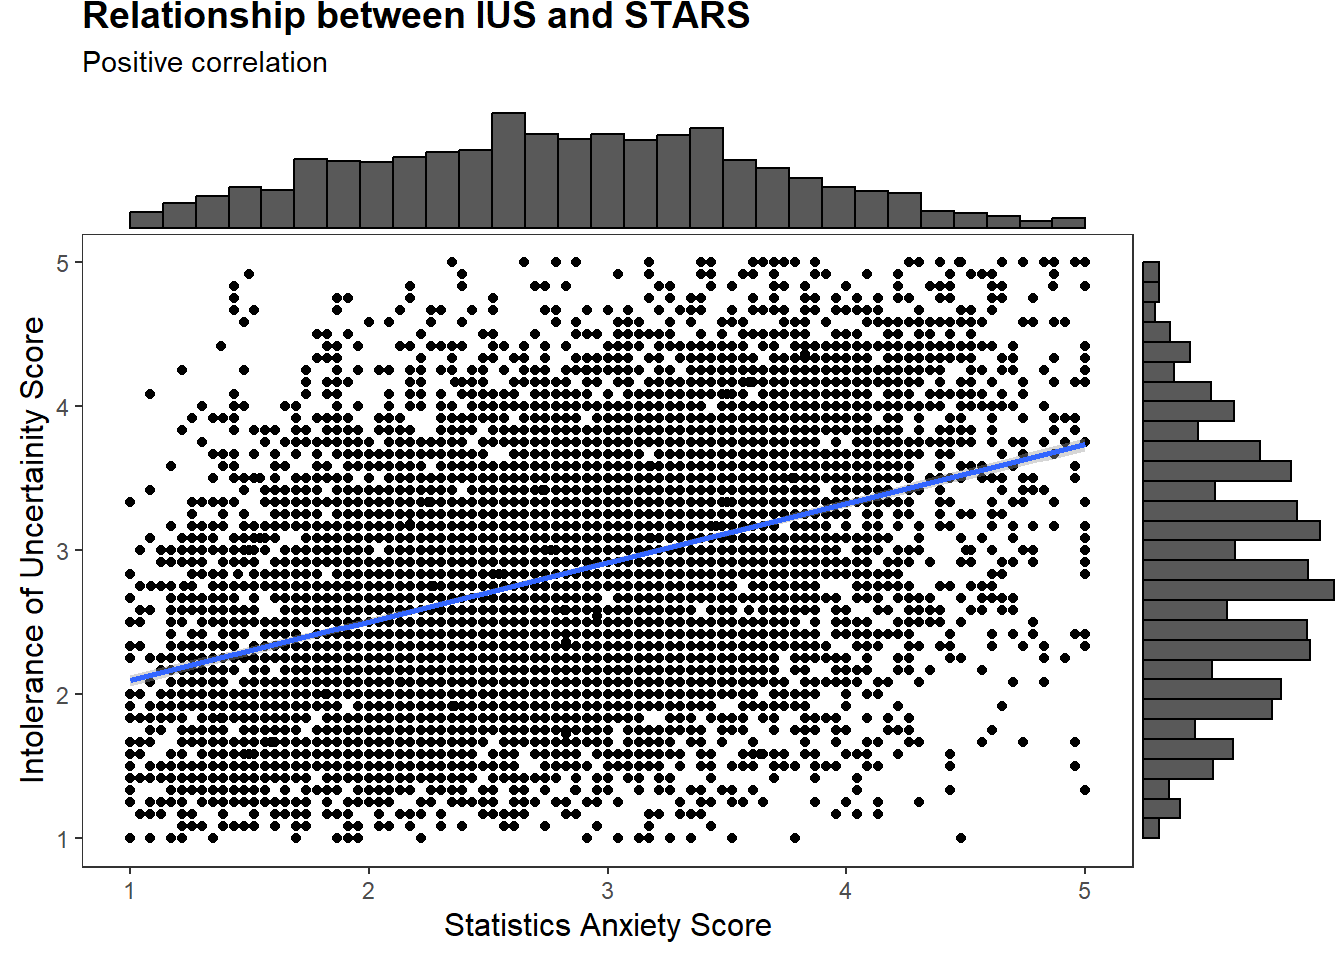
\includegraphics[width=1\linewidth]{02-webinar_files/figure-latex/unnamed-chunk-18-1} \end{center}

\section{FAQs}\label{faqs}

Before the webinar, you were given the opportunity to ask questions. Here are responses to the most frequent.

\subsection{What are the best resources for learning R as a beginner?}\label{what-are-the-best-resources-for-learning-r-as-a-beginner}

If you're a complete beginner and a psychology, I can recommend our own PsyTeachR collection:
- \href{https://psyteachr.github.io/data-skills-v3/}{Data Skills} is our 1st year undergrad course and is a very slow introduction to working in R, data wrangling, descriptives, and data viz
- \href{https://psyteachr.github.io/analysis-v3/}{Analysis} is our 2nd year UG resource and introduce inferential stats: chi-square, correlation, t-test, ANOVA, and regression
- \href{https://psyteachr.github.io/stat-models-v1/}{Statistical models} is our 3rd year UG resource and goes full GLM and introduces mixed effect models
- \href{https://psyteachr.github.io/quant-fun-v3/}{Fundamentals of Quantitative Analysis} is our one-year conversion course resource which is a compressed version of our 1st and 2nd year coverage.
- \href{https://psyteachr.github.io/ads-v3/}{Applied data skills} doesn't go into inferential stats,instead it's a deep dive into producing reproducible reports, data wrangling, transformation, and data viz.

For resources that weren't written by my team:

\begin{itemize}
\tightlist
\item
  \href{https://r4ds.hadley.nz/}{R for Data Science}
\end{itemize}

\subsection{What are the best resources specifically for data viz?}\label{what-are-the-best-resources-specifically-for-data-viz}

\begin{itemize}
\tightlist
\item
  \href{https://clauswilke.com/dataviz/}{Fundamentals of Data Visualization}
\item
  \href{https://socviz.co/}{Data Visualization: A practical introduction}
\item
  \href{https://bbc.github.io/rcookbook/\#how_to_create_bbc_style_graphics}{BBC Visual and Data Journalism cookbook for R graphics}
\item
  \href{https://r-graph-gallery.com/}{The R Graph Gallery}
\item
  \href{https://ggplot2-book.org/}{ggplot2: Elegant Graphics for Data Analysis (3e)}
\end{itemize}

\subsection{How can I use AI to help me learn to code}\label{how-can-i-use-ai-to-help-me-learn-to-code}

We've written a companion book: \href{https://psyteachr.github.io/AITutoR/}{AITutoR}

\subsection{How do you teach undergraduates R?}\label{how-do-you-teach-undergraduates-r}

The above links to our resources show you our materials and they allhave a Creative Commons licence so you can adpat and reuse them. I have also given a talk about our approach more broadly regarding teaching reproducible data skills: \href{https://osf.io/24c65}{slides here}.

\appendix


\chapter*{License}\label{license}
\addcontentsline{toc}{chapter}{License}

This book is licensed under Creative Commons Attribution-ShareAlike 4.0 International License \href{https://creativecommons.org/licenses/by-sa/4.0/}{(CC-BY-SA 4.0)}. You are free to share and adapt this book. You must give appropriate credit \citep{psyteachr-template}, provide a link to the license, and indicate if changes were made. If you adapt the material, you must distribute your contributions under the same license as the original.

  \bibliography{book.bib,packages.bib}

\end{document}
